%%%%%%%%%%%%%%%%%%%%%%%%%%%%%%%%%%%%%%%%%%%%%%%%%%%%%%%%%%%%%%%%%%%%%%%%%%%%%%%%%%%%%%%%%
%%                                                                                     %%
%%                This file is part of the CAPH Compiler distribution                  %%
%%                            http:%/caph.univ-bpclermont.fr                           %%
%%                                                                                     %%
%%                                  Jocelyn SEROT                                      %%
%%                         Jocelyn.Serot@univ-bpclermont.fr                            %%
%%                                                                                     %%
%%         Copyright 2011-2018 Jocelyn SEROT.  All rights reserved.                    %%
%%  This file is distributed under the terms of the GNU Library General Public License %%
%%      with the special exception on linking described in file ..%LICENSE.            %%
%%                                                                                     %%
%%%%%%%%%%%%%%%%%%%%%%%%%%%%%%%%%%%%%%%%%%%%%%%%%%%%%%%%%%%%%%%%%%%%%%%%%%%%%%%%%%%%%%%%%

\chapter{CAPH Overview}
\label{chap:overview}

This chapter introduces the \caph language. The basic structure of programs is presented. Its syntax
and semantics are introduced informally, by means of examples. Formal accounts can be found in
chapters~\ref{chap:syntax}, \ref{chap:abssyn}, \ref{chap:typing}, \ref{chap:static} and
\ref{chap:dynamic-semantics}.  In the examples, comments follow the \caph syntax : they are
single-line and starts with ``\texttt{--}''.

\section{Language structure}
\label{sec:language-struct}

As stated in introduction, \caph is a layered language. 

The outermost (\emph{declaration}) layer declares types, global values (constant and functions), I/O streams, actors and
network-level objects (wires and wiring functions).
The innermost (\emph{expression}) layer is used for describing computations. 
An \emph{actor} sub-language is used for describing the interface and the behavior of actors and a
\emph{network} sub-language is used for describing the structure of the dataflow process network. 

All layers essentially share a common type system, which is presented in the next section.

\section{Types}
\label{sect:types}

Broadly speaking, two categories of types can be distinguished: \emph{scalar} types and
\emph{structured} types\footnote{The concept of \emph{type variable} is discussed separately in
  Sec.~\ref{sec:polymorphism}}.

\subsection{Scalar types}
\label{sec:scalar-types}

Scalar types are described in Table~\ref{tab:scalar-types}. They include signed and unsigned
fixed-precision integers, booleans and floating-point values\footnote{Support of floating-point
  values by the VHDL backend is platform-dependant (see Sec.~\ref{sec:transl-syst-vhdl}).}.

\begin{table}
\small
\begin{center}
\begin{tabular}{|l|l|} \hline
\texttt{int} & Generic (signed) integer, range is implementation dependant\\ \hline   
\texttt{signed<prec>} & Sized signed integer, range is $-2^{prec-1}\ldots 2^{prec-1}-1$\\ \hline   
\texttt{unsigned<prec>} & Sized unsigned integer, range is $0 \ldots 2^{prec}-1$\\ \hline   
\texttt{bool}       & Boolean (\verb|true|, \verb|false|) \\ \hline   
\texttt{float}       & Floating-point value (minimal range : $-1.10^{38}\ldots+1.10^{38}$)  \\ \hline   
\end{tabular}
\caption{\caph scalar types}
\label{tab:scalar-types}
\end{center}
\end{table}

\medskip
Builtin operations provided on scalar types are summarized in Table~\ref{tab:scalar-ops}.
By \emph{builtin}, we mean the operations which
\begin{itemize}
\item have a runtime implementation at the simulator level,
\item can be a automatically translated to their SystemC and VHDL equivalent by the compiler
  back-ends\footnote{The support of floating-point values ultimately depends on the VHDL compiler.}.
\end{itemize}

\begin{table}
\begin{minipage}[c]{1.0\linewidth}
\small
\begin{center}
\begin{tabular}{|l|l|} \hline
{\tt bool}      & {\tt \&\& || not} (logical and, or, not) \\ \hline 
{\tt int}       & {\tt + - * / mod} \\ 
{\tt signed}    & \tt {< <= = >= >} \\
{\tt unsigned}  & \\ \hline
{\tt signed}    & {\tt land lor lnand lnot} (bitwise operations) \\
{\tt unsigned}  & {\tt <<}, {\tt >>} (left/right logical shift)\\  \hline
{\tt float}     & {\tt +. -. *. /.}  \\
                & {\tt =. !=. <. >. <=. >=.}  \\ \hline
%                & {\tt sll srl}\footnote{These operators can also be written {\tt <<} and {\tt >>} resp.} (left/right logical shift)\\ 
%                & {\tt sla sra} (left/right arithmetic shift)\\ 
%                & {\tt rol ror} (left/right rotate) \\ \hline
\end{tabular}
\caption{Builtin operations on scalar types}
\label{tab:scalar-ops}
\end{center}
\end{minipage}
\end{table}
\normalsize

% For \texttt{word}, {\verb+ & | ^ ~+} are bitwise and, inclusive or, exclusive or
% and negation respectively.  The {\tt <<} and {\tt >>} operations pad to right/left with
% {\tt 0}s respectively, as required.

\subsection{Structured types}
\label{sec:structured-types}

Two categories of structured types are currently supported : arrays and variants.

\bigskip \textbf{Arrays} are indexed collections of values of the same type. The corresponding type,
\texttt{array}, is predefined in \caph. Arrays can have one, two or three dimensions~:
\begin{itemize}
\item for 1D arrays, each item has a scalar type,
\item 2D arrays are viewed as arrays of 1D arrays\footnote{And for this reason, sometimes called
    1D$\times$1D arrays.},
\item 3D arrays are viewed as arrays of 2D arrays\footnote{And for this reason, sometimes called
    1D$\times$1D$\times$1D arrays.}.
\end{itemize}
For each dimension, the size $S$ is fixed and must defined at the declaration. Indexes range from
$0$ to $S-1$.

Arrays can be declared either as global constants or as local variables in actors
(Table~\ref{tab:array-decls}). In the first case, the (immutable) value of the array is part of the
declaration and an optional type signature can be used to refine the type of the array items. In the
second case, the type signature is not optional but the initial value can be omitted\footnote{It is
  the progammer's responsability, of course, to ensure that no element of the array will be accessed
  before having been properly initialized.}.  Two syntaxes -- extension and comprehension -- are
provided for specifying initilisation values. 

\begin{table}
\begin{minipage}[c]{1.0\linewidth}
\small
\begin{center}
\begin{tabular}{|l|r|} \hline
\texttt{const <id> "=" <array\_init> [ ":" <array\_type> ]} & global constant \\ 
\texttt{var <id> ":" <array\_type> [ "=" <array\_init> ]} & local variable \\ 
\emph{where} & \\
\texttt{<array\_init> ::=} & \\
\hspace{0.5cm}\texttt{<array\_ext1>} & 1D extension \\
\hspace{0.5cm}\texttt{<array\_ext2>} & 2D extension \\
\hspace{0.5cm}\texttt{<array\_ext3>} & 3D extension \\
\hspace{0.5cm}\texttt{| "[" <expr> "|" <index_range> "," ..., "," <index_range>} & comprehension \\ 
\texttt{<array_ext1> ::=} & \\
\hspace{0.5cm}\texttt{| "[" <scalar\_const>\_1 "," ... "," <scalar\_const>\_n "]"} & \\ 
\texttt{<array_ext2> ::=} & \\
\hspace{0.5cm}\texttt{| "[" <array\_ext1>\_1 "," ... "," <array\_ext1>\_n "]"} & \\ 
\texttt{<array_ext3> ::=} & \\
\hspace{0.5cm}\texttt{| "[" <array\_ext2>\_1 "," ... "," <array\_ext2>\_n "]"} & \\ 
\texttt{<index\_range> ::=} & \\
\hspace{0.5cm}\texttt{| <id> "=" <index\_1> "to" <index\_2>} & \\ 
\emph{and} & \\
\texttt{<array\_type> ::=} & \\
\hspace{0.5cm}\texttt{<scalar\_type> "array" "[" <size> "]"} & 1D array \\
\hspace{0.5cm}\texttt{<scalar\_type> "array" "[" <size> "]" "[" <size> "]"} & 2D array \\
\hspace{0.5cm}\texttt{<scalar\_type> "array" "[" <size> "]" "[" <size> "]" "[" <size> "]"} & 3D array \\
\emph{Examples} & \\
\texttt{var a : signed<4> array[4]} & \\
\texttt{var b : unsigned<8> array[4] = [1,2,3,4]} & \\
\texttt{var c : unsigned<8> array[4] = [i*2 | i=0 to 3]}\footnote{This is equivalent to \texttt{var
    c : unsigned<8> array[4] = [0,2,4,6]}} & \\ 
\texttt{const a1 = [1,2,3,4] : signed<4> array[4]} & \\
\texttt{const a2 = [[1,2],[3,4],[5,6]] : signed<4> array[3][2]} & \\
\texttt{const a3 = [[[1,2],[3,4]],[[5,6],[7,8]]] : signed<4> array[2][2][2]} & \\ \hline
\end{tabular}
\caption{Array declarations}
\label{tab:array-decls}
\end{center}
\end{minipage}
\end{table}

Individual array items can be accessed for reading and updating using the classical \verb|[.]| notation
(Table~\ref{tab:array-exprs}). 

\begin{table}
\begin{minipage}[c]{1.0\linewidth}
\small
\begin{center}
\begin{tabular}{|l|r|} \hline
\texttt{<array\_id>"["<index\_expr>"]"} & for 1D arrays \\ 
\texttt{<array\_id>"["<index\_expr>"]" "["<index\_expr>"]"} & for 2D arrays \\ 
\texttt{<array\_id>"["<index\_expr>"]" "["<index\_expr>"]" "["<index\_expr>"]"} & for 3D arrays \\ 
\emph{where} & \\
\texttt{<index\_expr>} is any expression of type \texttt{int} & \\
\emph{Examples} & \\
\texttt{t[1]} & \\
\texttt{t[2*i+1]} & \\
\texttt{t[i][j]} & \\
\texttt{t[i][j][2]} & \\ \hline
\end{tabular}
\caption{Array expressions}
\label{tab:array-exprs}
\end{center}
\end{minipage}
\end{table}


% \begin{table}
% \begin{minipage}[c]{1.0\linewidth}
% \small
% \begin{center}
% \begin{tabular}{|l|l|l|} \hline
% Array declaration & \texttt{<scalar\_type> <array\_id>"["<size>[","<size'>]"]" [ "=" <array\_init> ]} \\ 
%                   & ex: \texttt{signed<4> a[4]} \\
%                   & ex: \texttt{signed<4> b[4] = [1,2,3,4]} \\
%                   & ex: \texttt{unsigned<8> c[4] = [i in 0..3 <- i*2]}\footnote{This is equivalent to \texttt{unsigned<8> c[4] = [0,2,4,6]}} \\ 
%                   & ex: \texttt{unsigned<8> c[256] = [0:256]}\footnote{This is equivalent to
%                     \texttt{unsigned<8> c[256] = [i in 0..255 <- 0]}} \\ 
%                   & ex: \texttt{signed<8> d[2,2] = [[1,2],[3,4]]} \\
%                   & ex: \texttt{signed<8> d[2,2] = [i in 0..1, j in 0..1 <- if i=j then 1 else
%                     0]}\footnote{This is equivalent to \texttt{signed<8> d[2,2] = [[1,0],[0,1]]}} \\ \hline
% Array access & \texttt{<array\_id>"["<index\_expr>"[","<index\_expr>]"]"} \\ 
%             & ex: \texttt{v := a[2]} (1D case) \\
%             & ex: \texttt{v := d[0,1]} (2D case) \\ \hline
% Array ``update'' & \texttt{<array\_id>"["<index\_expr1>"<-"<expr1>","...","<index\_exprN>"<-"<exprN>"]"} \\ 
%                  & \texttt{<array\_id>"["<id1> "in" <range1>","...","<idN> "in" <rangeN> "<-" <expr>"]"} \\ 
%              & ex: \texttt{a := b[1<-8]}\footnote{$a_i=b_i\ \forall i\not= 1, a_1=8$} \\ 
%              & ex: \texttt{b := b[1<-8,2<-6]}\footnote{$b_0=1,b_1=8,b_2=6,b_3=4$} \\ \hline
%              & ex: \texttt{b := b[i in 1 .. 2 <- b[i]*2]}\footnote{$b_0=1,b_1=16,b_2=12,b_3=4$} \\ \hline
% \end{tabular}
% \caption{Operations on arrays}
% \label{tab:array_ops}
% \end{center}
% \end{minipage}
% \end{table}

% \medskip \textbf{Vectors} are used to define higher-order wiring functions at the
% coordination level. They are only available at the coordination level.
% \tbw

\bigskip \textbf{Variants} allow values of different
kinds to be mixed together in a common type by tagging them with a distinct label. They are
described in Sec.~\ref{sec:type-declarations}.

\subsection{Translation to SystemC and VHDL types}
\label{sec:transl-syst-vhdl}

Table~\ref{tab:type-transl} describes how \caph types are translated to SystemC or VHDL types by the
compiler back-ends.

In VHDL, Tokens circulating between actors are represented as
\texttt{std\_logic\_vector}s and numeric values are represented using the
\texttt{signed} or \texttt{unsigned} data types defined in the \texttt{ieee.numeric\_std}
library\footnote{There's a compiler option to change the default library used for implementing
  arithmetic operations.}. Booleans are encoded as VHDL \texttt{boolean}s. Floating-point values are
currently encoded using the \texttt{float32} type provided by the \emph{VHDL-2008 Support Library} available
at \texttt{http://www.vhdl.org/fphdl}\footnote{This should be viewed as a temporary solution, before
  the full VHDL-2008 standard is supported by mainstream VHDL compilers and synthetizers. Support
  for floating-point values can be disabled if this library cannot be installed on the target
  platform.}.

\begin{table}
\begin{minipage}[c]{1.0\linewidth}
\small
\begin{center}
\begin{tabular}{|l|l|l|} \hline
\caph                  &  SystemC                &  VHDL \\ \hline
\texttt{bool}          & \texttt{bool}           & \texttt{boolean} \\ \hline
\texttt{int}           & \texttt{int}            & \texttt{signed<prec-1 downto 0>} \\ \hline
\texttt{signed<prec>}& \texttt{sc\_int<prec>} or \texttt{int}\footnote{Depending on whether
  \texttt{prec} resolves to a static constant or not.}   & \texttt{signed<prec-1 downto 0>} \\ \hline
\texttt{unsigned<prec>}& \texttt{sc\_uint<prec>} or \texttt{unsigned int}\footnote{Depending on whether
  \texttt{prec} resolves to a static constant or not.}   & \texttt{unsigned<prec-1 downto 0>} \\ \hline
\texttt{float}         & \texttt{float}\footnote{C native \texttt{float} type (32 bits)}   & \texttt{float32}\\ \hline
\texttt{t array[sz]}\footnote{Where \texttt{t} is a scalar type.}  & \texttt{std::array<t',sz>}  & \texttt{array (0 to sz-1) of t'} \\
                         &                           & \hspace{1cm}where \texttt{t'} is translation of type \texttt{t} \\ \hline
\texttt{t array[sz][sz']}\footnote{Where \texttt{t} is a scalar type.}  &
\texttt{std::array<std::array<t',sz>,sz'>}  &
\texttt{array (0 to sz-1) of array (0 to sz'-1) of t'} \\
                         &                           & \hspace{1cm}where \texttt{t'} is translation of type \texttt{t} \\ \hline
%\texttt{t array<sz1,sz2>}\footnote{Where \texttt{t} is a scalar type.}  & C array   & \texttt{array
%  (0 to sz1-1, 0 to sz2-2)  of t'} \\
%                        &                            & \hspace{1cm}where \texttt{t'} is translation of type \texttt{t} \\ \hline
\texttt{t}\footnote{Where \texttt{t} is a variant type.}  & \texttt{class} \ldots\footnote{See
  chapter~\ref{cha:variants-impl}.} & \texttt{std\_logic\_vector<m+n>} \\
              &         & where  \\
              &         & $m=\lceil log_2 N_c \rceil$ \\
              &         & $n=max_{i=1\ldots N_c}|\tau_i|$ \\
              &         & $N_c$ is the number of distinct tags \\
              &         & $\tau_i$ is the type of argument for tag $i$ \\
              &         & $|\tau|$ is size (in bits) of the VHDL representation for type $\tau$ \\
              &         & The $m$ MSBs are used to encode the tag. \\
              &         & The $n$ LSBs are used to encode the argument\footnote{See
                chapter~\ref{cha:variants-impl}.} \\ \hline
%\texttt{t vector}\footnote{Where \texttt{t} is \texttt{int} or \texttt{bool}.}  &
%N/A\footnote{Vectors are only used to define wiring functions. They are never manipulated
%  by actors.}  & N/A \\ \hline
\end{tabular}
\caption{Translation of types in SystemC and VHDL}
\label{tab:type-transl}
\end{center}
\end{minipage}
\end{table}

\section{CAPH expression language}
\label{sec:caph-expr-lang}

The expression language is a small, purely functional, first-order, polymorphic language with a strict
semantics. This language is used both for defining the values assigned to global constants and
functions at the declaration level and the values computed when a rule is fired at the actor level.
Its syntax broadly follows that of Caml~\cite{Caml}.

The expression language cannot manipulate functions as values, like in classical, higher-order
functional languages. This makes sense since this concept cannot be translated, in general, into
hardware.

\subsection{Constants}
\label{sec:e-constants}

Constants at the expression-level are simple constant values covering the basic \caph types
(integers and booleans). By default, integer constants are un-signed and un-sized. Signness and size
can be provided using the type coercion operator "\verb|:|" (see Sec~\ref{sec:e-coerce}). Signness
can also specified using the \verb|U| and \verb|S| suffixes or implicitely for negative ints.

\begin{lstlisting}[title=Example]
23                 -- generic int
23S                -- signed int
23U                -- unsigned int
-12                -- signed int
(12:unsigned<4>)   -- sized, unsigned int
(12:signed<8>)     -- sized, signed int
true               -- boolean
0xFA               -- hex constant
0b1001             -- binary constant
1.23               -- float constant
-2.3               -- float constant
\end{lstlisting}

Type coercion can be used to define constants with a more precise type (see Sec~\ref{sec:e-coerce}).

\subsection{Variables}
\label{sec:e-variables}

Variables appearing at the expression level are simple identifiers. These identifiers must have
been bound at the declaration layer or with an upper \texttt{let} declaration within the same
expression. Identifiers must start with a lowercase letter (symbols starting with
an uppercase letter are used to designate data constructors).

\subsection{Function application}
\label{sec:e-fun-app}

Functions are always fully applied at the expression level\footnote{This is to be contrasted to functions
  defined at the network level, where higher-order functions and partial application are supported.}. The applied
function must have been declared in the declaration layer or be a builtin primitive. Application
of builtin primitives uses the classical infix notation.

%\noindent \textbf{Example}\xrfill{.5pt}
\begin{lstlisting}[title=Example]
g (3)          -- g is function with arity 1
f (1,2)        -- f is function with arity 2
1+2            -- + is a builtin primitive
\end{lstlisting}
%\noindent \xrfill{.5pt}

\subsection{Conditionals}
\label{sec:conditionnals}

Conditional expressions always have two alternatives, depending on
the value of the discriminating expression is ({\tt true} or {\tt false}).

\begin{lstlisting}[title=Example]
if x>1 then x-1 else x
\end{lstlisting}

\subsection{Local Declarations}
\label{sec:let-decls}

Local declarations are used to bind variable(s) to expression(s) within the (limited) scope of a given
expression. The names introduced by the bindings are only visible within the target
expression. Bindings are evaluated before the target expression is evaluated.

\begin{lstlisting}[title=Example]
let x=1+2 in x*x              -- expression value is 9
let x=1+2 and y=3*4 in x+y    -- expression value is 15
\end{lstlisting}

Local declarations can be nested. This offers a way for ``breaking'' complex computations and/or
sharing intermediary results. 

\begin{lstlisting}[title=Example]
let y=2*x+1 in let z=y*y-5 in z/4
\end{lstlisting}

\noindent
The previous example is equivalent to writing \texttt{((2*x+1)*(2*x+1)-5)/4}.

\subsection{Type coercion}
\label{sec:e-coerce}

The expression language has a builtin operator (\texttt{:}) for performing type coercion.
Type coercion is often necessary to assign values a more ``precise'' type than that infered by the
type checker in order to provide the compiler back-ends enough information. 


\begin{lstlisting}[title=Example]
(1+2 : unsigned<8>)
\end{lstlisting}

Here the type inferred by the type-checker for the mere expression \texttt{1+2} is simply
the \emph{generic} type \texttt{int}\footnote{In fact, this is
  \texttt{int<s,n>} where \texttt{s} and \texttt{n} are respectively a \emph{sign variable} and a
  \emph{size} variable. The notion of type variable is discussed in Sec.~\ref{sec:polymorphism}.}. This type is
here explicitely refined to \texttt{unsigned<8>}\footnote{Where \texttt{unsigned<8>} is actually an
  abbreviation for \texttt{int<_unsigned,8>}.}.

The coercibility relation between base types is described in Table~\ref{tab:type-casting}. A \emph{S} at
intersection of row \texttt{t} and column \texttt{t'} means that type \texttt{t} can be safely
coerced to type \texttt{t'} (with no loss of information); a \emph{U} (unsafe) indicates that some information
may be lost and a \emph{F} indicates a forbidden operation.

This relation naturally extends to structured types with the same constructor and the same number of
elements. For example, type \texttt{t array[m]} can be coerced to \texttt{t' array[n]} iff
\texttt{m=n} and \texttt{t} can be coerced to \texttt{t'}.

Coercion between integer types is only accepted in two situations:
\begin{enumerate}
\item  it corresponds to a ``refinement'' of the LHS type. Examples :
  \begin{itemize}
  \item \verb|(int<8>:unsigned<8>)| is ok,
  \item \verb|(int:unsigned<8>)| is ok,
  \item \verb|(signed<n>:signed<16>)| (where \verb|n| is an unbound size variable) is ok,
  \item \verb|(unsigned<8>:int)| is forbidden,
  \item \verb|(signed<8>:signed<n>)| (where \verb|n| is an unbound size variable) is forbidden\footnote{The known size 8 cannot be ``erased''.}.
  \end{itemize}
\item it corresponds to a modification of an already known signness or size. Examples
  \begin{itemize}
  \item \verb|(signed<8>:signed<16>)| is ok 
  \item \verb|(signed<8>:unsigned<8>)| is ok (but the sign is lost),
  \item \verb|(unsigned<16>:unsigned<8>)| is ok (but the result may be truncated).
  \end{itemize}
\end{enumerate}
The compiler accepts coercions of the first kind silently and emits a warning for the second kind 
when the signness/sizes of the LHS and RHS is/are different.

\begin{table}
\begin{minipage}[c]{1.0\linewidth}
\small
\begin{center}
\begin{tabular}{|c|c|c|c|c|c|} \hline
                     & \texttt{bool}     & \texttt{int}      & \texttt{signed<n>}   & \texttt{unsigned<n>}  & \texttt{float}    \\ \hline
\texttt{bool}        & S                 & S\footnotemark[1] & S\footnotemark[1]    & S\footnotemark[1]     & S\footnotemark[1] \\ \hline
\texttt{int}         & U\footnotemark[2] & S                 & S                    & S                     & S \\ \hline
\texttt{signed<m>}   & U\footnotemark[2] & F                 & U\footnotemark[3]    & U\footnotemark[4]     & S \\ \hline
\texttt{unsigned<m>} & U\footnotemark[2] & F                 & U\footnotemark[5]    & U\footnotemark[3]     & S \\ \hline
\texttt{float}       & U\footnotemark[2] & U\footnotemark[7] & U\footnotemark[7]    & U\footnotemark[7]     & S \\ \hline
\end{tabular}
\caption{Type casting between base types}
\label{tab:type-casting}
\end{center}
\footnotetext[1]{\texttt{true} is translated to 1, \texttt{false} to 0.}
\footnotetext[2]{0 is translated to \texttt{false}, all other values to \texttt{true}.}
\footnotetext[3]{Truncature may occur if $m>n$}
\footnotetext[4]{Sign is lost. Truncature may occur if $m>n$}
\footnotetext[5]{Truncature may occur if $m>n-1$}
\footnotetext[6]{Some loss of precision may occur}
\footnotetext[7]{The fractional part is discarded. Truncature may occur}
\end{minipage}
\end{table}

\subsection{Attributes}
\label{sec:attributes}

An \emph{attribute} is a property which can be attached to certain types of value.  Examples
are the size (number of elements) of an arrays or the width (in bits) of an integer value.

\medskip
Attribute values can be retrieved using the following syntax : \verb|<value_name>`<attribute_name>|.

\medskip
A typical use is of attributes is for initializing arrays :

\begin{lstlisting}[title=Example]
var z : array[8] = [ 0 | i=0 to z`size-1 ]
\end{lstlisting}

The current version of the compiler only supports one kind of the attribute, named \verb|size|. The
meaning of this attribute directly depends on the \emph{type} of the value to which it is
attached. Table~\ref{tab:size-attr} gives its interpretation for all \caph builtin
types\footnote{The value of the \texttt{size} attribute is undefined for user-defined types.}. 

\begin{table}
\begin{center}
\begin{tabular}{|l|l|} \hline
If value \texttt{v} has type\ldots  &  \verb|v`size| gives\ldots  \\ \hline
\texttt{bool}          & 1 \\ \hline
\texttt{int<prec>}     & \texttt{<prec>} \\ \hline
\texttt{signed<prec>}& \texttt{<prec>}  \\ \hline
\texttt{unsigned<prec>}& \texttt{<prec>}  \\ \hline
\texttt{float}         & 32 \\ \hline
\texttt{t array[sz]}   & \verb|sz| \\ \hline
$\tau_1 \times \ldots \times \tau_n$            & $n$ \\ \hline
\end{tabular}
\caption{Interpretation of the \texttt{size} attribute}
\label{tab:size-attr}
\end{center}
\end{table}

\section{CAPH declaration language}
\label{sect:declaration-language}

This is the outermost layer. A \caph program is just a sequence of \emph{declarations}, which are
evaluated sequentially (in other words, the declaration of an object may refer to objects declared
before but not the other way).  Declarations concerns declares types, global values (constant and
functions), I/O streams, actors and network-level objects (wires and wiring functions).

\subsection{Type declarations}
\label{sec:type-declarations}

There are two kinds of type declarations : type synonym declarations and variant declarations.

\bigskip \textbf{Type synonym declarations} are used to introduce abbreviations to existing types.
For example, the following declaration defines a type \texttt{byte} which is a synonym to the
builtin type \verb|unsigned<8>| : 

\begin{lstlisting}[title=Example]
type byte == unsigned<8>;  -- byte is now a synomym for unsigned<8>
\end{lstlisting}

\bigskip \textbf{Variant declarations} are used to define \emph{algebraic data types}. These types
-- also called \emph{tagged unions} -- allow values of different types to be mixed together by
tagging them with a distinct label.  Consider for example the situation in which a token can carry
either a signed or unsigned 8-bit value. A type for this kind of tokens could be defined with the
following type declaration :

\begin{lstlisting}[]
type us8 = 
    Signed of signed<8> 
  | Unsigned of unsigned<8> 
\end{lstlisting}

This declaration introduces the \emph{type constructor} \verb|us8|. A value of type \verb|us8| is
either a \verb|signed<8>| value or a \verb|unsigned<8>| value. The associated tag (\verb|Signed| or
\verb|Unsigned|) is used to distinguish between these two cases.

More generally speaking, the declaration of a variant type lists all possible ``shapes'' for values of
that type. Each case is identified by a specific tag, called a \emph{value constructor}, which serves both for
constructing values of the variant type and inspecting them by pattern-matching (see
Sec.~\ref{sec:actor-examples} for examples). Value constructors can take $0$ to $n$
arguments\footnote{Since version 2.6.2. In previous versions only nullary and unary value
  constructors were supported.}. To distinguish them from variable names -- which start with a
lowercase letter -- they must start with a capital letter.

\medskip
Type constructors can be polymorphic, \ie they can be parameterized over (an)other type(s), called the
\emph{argument types(s)} (see Sec.~\ref{sec:polymorphism}). For example, here's a definition of a type
for representing \emph{optional} values (\ie values that can be either present or absent) :

\begin{lstlisting}[title=Example 1]
type $t option = 
  Absent
| Present of $t
\end{lstlisting}

A value of type \mbox{$\tau$ \texttt{option}} is either \verb|Absent| or \verb|Present v|, where
\verb|v| is a value of type $\tau$ and $\tau$ can be any type.

\medskip
The following definition introduces a type for representing optionally labeled values~:

\begin{lstlisting}[title=Example 2]
type ($t1,$t2) labeled  = 
| Unlabeled of $t1
| Labeled of $t1 * $t2
\end{lstlisting} % $

A value of type \mbox{$(\tau,\lambda)$ \texttt{labeled}} is either \verb|Unlabeled v|, where
\verb|v| is a value of type $\tau$ or \verb|Labeled (v,l)| where \verb|v| is a value of type $\tau$
and \verb|l| a value of type $\lambda$. As above, $\tau$ and $\lambda$ can be any type.

\medskip
When an variant type involves sized integers, it can be parameterized over the corresponding sizes. 
The size parameters are then specified by listing them, between \verb|<| and \verb|>| after the name
of the type constructor\footnote{This ``hybrid'' approach, in which \emph{type} parameters are
  specified using a prefix notation and \emph{size} parameters using a postfix notation may appear 
  awkward to programmers familiar to purely prefix (OCaml, for example) of purely postfix-based
  (C++, for example) notations. It has been chosen because different trials have shown us that the
  other choices actually led to slightly more verbose
  formulations to avoid parsing ambiguities.}
For example, the type \verb|us8| introduced above could be generalized as follows : 
matter
\begin{lstlisting}[]
type us<n> = 
    Signed of signed<n> 
  | Unsigned of unsigned<n> 
\end{lstlisting}

The type \verb|us| can now be used to represent values having type \verb|signed<n>| or
\verb|unsigned<n>|, where \verb|n| can be any possible value. 

\medskip 
The two kinds of polymorphism (type and size) can appear in the same declaration. Here's for example
the declation of a type \verb|tau| whose values are either a signed integers with size \verb|n| or values of
type \verb|t| :

\begin{lstlisting}[]
type $t tau<n> = 
    Left of signed<n> 
  | Right of $t
\end{lstlisting}

\bigskip
The \caph standard library defines (in \verb|lib/caph/dc.cph|) the following type\footnote{This type
  was builtin in versions prior to 2.6.2.}~:

\begin{lstlisting}[frame=none]
type $t dc = 
  Data of $t
| SoS
| EoS
\end{lstlisting}

 \medskip The \textbf{dc} type (abbreviation for \emph{data/control}) can be used to encode
 \emph{structured streams}, \ie streams in which the sequence of tokens obeys to a certain structure
 (as opposed to ``raw'' streams in which the only structure is the order in which tokens
 appears). Consider for example the stream representing a (potentially infinite) sequence of $n
 \times n$ images. Representing this sequence as a simple stream of tokens, where each token carries
 a pixel value is generally not sufficient. Most often, actors operating on this stream will need to
 detect the start and end of a single image in this stream and the start and end of individual lines
 in this image.  This need to \emph{structure} the stream of tokens can be served by dividing the
 tokens, circulating on channels and manipulated by actors, into two broad categories : \emph{data}
 tokens (carrying actual values) and \emph{control} tokens (acting as structuring delimiters). For
 the aforementionned example, one could therefore introduce the following type to represent
 sequences of images :

\begin{lstlisting}[title=Example]
type $t image =
  | SoI            -- Start of image
  | EoI            -- End of image
  | SoL            -- Start of line
  | EoL            -- End of line
  | Data of $t    -- Pixel
\end{lstlisting}

Tokens with values \verb|SoI|, \verb|EoI|, \verb|SoL| and \verb|EoL| will be control tokens
indicating the start and end of images (resp. lines) and pixels will be carried by tokens having
values \verb|Data v|. With the scheme, the $4 \times 4$ image of Fig.~\ref{fig:img4} may be represented by the following
stream of tokens:

%\footnotesize
\begin{center}
\begin{spverbatim}
SoI, SoL, Data(10), Data(30), Data(55), Data(90), EoL,
     SoL, Data(33), Data(53), Data(60), Data(12), EoL,
     SoL, Data(99), Data(56), Data(23), Data(11), EoL,
     SoL, Data(11), Data(82), Data(46), Data(11), EoL,  EoI
\end{spverbatim}
\end{center}
\normalsize

But it turns out that the type introduced above is sufficient for performing this encoding
of images as structured streams. The idea is that an image can viewed as a \emph{list} of lines,
where each line can in turn be viewed as a \emph{list} of pixels. For this, the \verb|SoS|
(resp. \verb|EoS|) is interpreted as a \emph{start of list} (resp. \emph{end of list}) control
token, and the $4 \times 4$ image of Fig.~\ref{fig:img4} is now represented by the following
stream of tokens:

%\footnotesize
\begin{center}
\begin{spverbatim}
SoS, SoS, Data(10), Data(30), Data(55), Data(90), EoS,
     SoS, Data(33), Data(53), Data(60), Data(12), EoS,
     SoS, Data(99), Data(56), Data(23), Data(11), EoS,
     SoS, Data(11), Data(82), Data(46), Data(11), EoS,  EoS
\end{spverbatim}
\end{center}
\normalsize

The advantage\footnote{Which has probably not escaped to programmers familiar with the Lisp
language\ldots} is that any kind of data structure can be represented this way : images, lists, but
also trees, \emph{etc.}, without requiring dedicated types.  

Moreover,
this structured representation of data nicely fits the stream-proces\-sing programming and execution
models.
Since the structure of the data is explicitly contained in the token stream no global control
  and/or synchronization is needed; this has strong and positive consequences both at the
  programming level (it justifies \emph{a posteriori} the style of description we introduced in the
  previous subsection for actors) and the execution level (it will greatly eases the production of
  HDL code).
Moreover, it naturally supports a pipelined execution scheme; processing of a line by an actor, for
  example, can begin as soon as the first pixel is read without having to wait for the entire structure
  to be received; this feature, which effectively allows concurrent circulation of successive
  ``waves'' of tokens through the network of actors is of course crucial for on-the-fly processing
  (like in real-time image processing).

\begin{figure}[h]
  \centering
  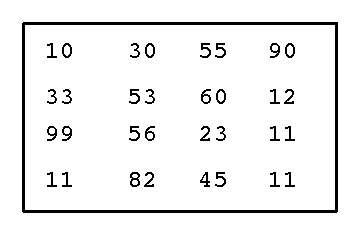
\includegraphics[width=4cm]{figs/datarepr}
  \caption{A $4 \times 4$ image}
  \label{fig:img4}
\end{figure}

\subsection{Value declarations}
\label{sec:value-declarations}

There are two types of value declarations : constants and functions.

Identifiers bound in these declarations scope over both the actor and network sub-languages, but
an important distinction must be made.

At the actor level, they can appear everywhere in the expressions defining the behavior of actors
(in the right-hand side of actor rules -- see Sec.~\ref{sec:actor-body}).  As a matter of fact,
global functions are often used to improve the readability of actors, by allowing a separation
between purely combinational and sequential aspects.

At the network level, they can only appear as parameters when an actor is instanciated (see
Sec~\ref{sec:network-expressions}) and cannot be used to define network-level expressions.

\subsubsection{Constant declarations}
\label{sec:const-decl}

Constant declarations are like \texttt{\#define} declarations in C. They give a name to a value which
is computed statically. They are typically used to define application-specific parameters.

\begin{lstlisting}[title=Example]
const threshold = 1+2;                -- scalar constant
const kernel = [1,2,1];               -- 1D array constant 
const kernels = [[1,2,1],[1,4,1]];    -- 1Dx1D array constant 
\end{lstlisting}

\subsubsection{Function declarations}
\label{sec:funct-decl}

Function declarations introduce functions, mapping an identifier (or a set of
identifiers) to an expression. Functions with several arguments are represented as functions taking a tuple. 
An optional type signature can be specified to refine the type of the function.

\begin{lstlisting}[title=Example]
function incr x = x+1;
function scale (x,s) = x*s : signed<8> * signed<8> -> signed<16>;
\end{lstlisting}

\subsubsection{External function declarations}
\label{sec:extern-funct-decl}

External functions declarations introduce functions which are defined outside the \caph language.
Their main usage is to allow the SystemC or VHDL generated code to make use of pre-existing
functions already written in these languages. The type of the corresponding function must be
supplied. For the corresponding program to be simulated, a Caml
implementation of the function must also be provided\footnote{It could be possible to interface the
  simulator directly to the C code but this is not currently implemented. Hence the necessity to
  provide the Caml version of the function.}.

\begin{lstlisting}[title=Example]
function sqrt x =
  extern "sqrt_c","sqrt_vhd","sqrt_ml": unsigned<16> -> unsigned<16>;
\end{lstlisting}

In the above example, \texttt{sqrt\_c}, \texttt{sqrt\_vhd} and \texttt{sqrt\_ml} are the names of
the C, VHDL and Caml implementations of the \texttt{sqrt} \caph function\footnote{We have used three
different names but in practice, the same name can be used for the three implementations.}. 
These functions are supposed to be defined in a file accessible when compiling the code generated by
the back-ends. For the ML function, it must be defined in a specific file and registered using a
dedicated function. The mechanism is detailed in Chap.~\ref{cha:foreign-funct-interf}

Its the programmer's responsability to ensure that the actual types of the function arguments and result
are compatible with the types specified in the declaration. There's currently no specific type-based
translation mechanism for foreign values. As a result, only functions whose arguments and result can
be safely coerced to integers are supported.

\subsection{I/O declaration}
\label{sec:io-declarations}

These declarations specify the way by which the application will interact with the operating system
(during simulation) or the physical devices (for the generated VHDL code for example).

Two types of I/Os are supported : \texttt{stream}s and \texttt{port}s.

\medskip
Streams are used to model pure data flows, in which tokens are read (resp. written) from (resp. to)
a sequential source (resp sink) using a fifo-like protocol. 

\medskip
Ports are used to model ``asynchronous'' I/Os, in which values are read (resp. written) using a
RAM-like interface.

\medskip
Both types of declarations specify a name, a type, a direction (input or output) and a
``device''. The device is a system-specific designator identifying the entity the input
(resp. output) data will be read from (resp. written to). When using the simulator, designators will
be simple file names. The SystemC and VHDL backends may use more system and platform specific designators. 
For port inputs, the declaration also specify an initial value\footnote{For port inputs, the device can be omitted; in
this case the port behaves as a constant generator.}. 

\begin{lstlisting}[title=Example]
stream inp1 : unsigned<8> from "sample.txt";
stream outp : signed<8> to "display:0";

port inp2: unsigned<16> from "threshold.txt" init 64;
port inp3: signed<8> init -1;
port outp2: boolean to "acks.txt";
\end{lstlisting}

\subsection{Actor declarations}
\label{sec:actor-declarations}

Each actor involved in the dataflow process network must be declared. The declaration comprises an
\emph{interface} (which is the only visible part at the network level) and a \emph{body}, describing
its behavior.

\subsubsection{Actor interface}
\label{sec:actor-interface}

The interface specifies the actor input(s), output(s) and optional parameter(s). All inputs, outputs
and parameters are typed. When building the network, inputs and outputs will be connected to
channels and parameters will be given values.

\begin{lstlisting}[title=Example]
-- This actor has one input, of type int, one output, of type bool and no parameter

actor a1
  in (x: int)
 out (y: bool)
 --  ...  actor body ...
\end{lstlisting}

\begin{lstlisting}[title=Example]
 -- This actor has two inputs, both of type signed<8>, one output, of type signed<8> and one parameter, of type unsigned<4>

actor a2 (k:unsigned<4>)
  in (e1: signed<8>, e2: signed<8>)
 out (s: signed<8>)
 --  ...  actor body ...
\end{lstlisting}

\subsubsection{Actor body}
\label{sec:actor-body}

The actor body comprises a set of local variable declarations and a set of transition rules.

\medskip
The set of \textbf{local variable declarations} can be empty. Each variable is declared with a name, a type and an
optional initial value. Variables are used to retain values between successive activations of the
actor. Their scope is limited to the actor they are defined in.

\medskip
In addition to the types defined in Sec.~\ref{sect:types}, local variables can also have an
\emph{enumerated} type. Two kinds of enumerated type are accepted : explicit enumerations  and
integer ranges.

\medskip Explicit enumerations are actually variant types for which all constructors have arity 0. 

\begin{lstlisting}[title=Example]
actor ...
 ...
var state : { S0, S1, S2 }
...
\end{lstlisting}

Declaring a local variable with such a type \emph{de facto} introduces a new type but
the corresponding type constructor is anonymous 
and the scope of the introduced data constructors (\texttt{S0}, \texttt{S1}, \ldots) is limited to
  the englobing actor\footnote{This feature was introduced precisely to avoid name conflicts that
    frequently arise if one has to declare global type and data constructors for locally defined
    values such as state variables.}.

\medskip Integer ranges may be viewed as a subset of the \verb|int| type.

\begin{lstlisting}[title=Example]
actor ...
 ...
var ctr : { 1,..,8 };
...
\end{lstlisting}

A variable with such a type can be used in any expression in which an \verb|int| can be
accepted. The main distinction is that it will be recognized as a potential
\emph{state} variable when performing abstract interpretation or FSM dumping (see
Sec.~\ref{sec:dumping-box-fsm} and chapter~\ref{cha:moc}). 

\bigskip
The behavior of an actor is specified using a set of \textbf{transition rules}. 

Each rule consists of a set of \emph{patterns}, involving inputs and local variables, and a set of
\emph{expressions}, describing modifications of outputs and/or local variables.

Each rule has the form

\begin{center}
$|\quad (\text{qual}_1:\text{pat}_1, \ldots, \text{qual}_m:\text{pat}_m) \rightarrow (\text{qual'}_1:\text{exp}_1, \ldots, \text{qual'}_n:\text{exp}_n)$
\end{center}

where
\begin{itemize}
\item $qual$ designates an input, a scalar variable or an element of an array variable,
\item $pat$ is a pattern,
\item $qual'$ designates an output, a scalar variable or an element of an array variable,
\item $exp$ is an expression.
\end{itemize}

Parens can be omitted if $m=1$ (resp. $n=1$).

\medskip
A pattern can be 
\begin{itemize}
\item a litteral constant\footnote{Constants defined in value declaration section (see
    Sec.~\ref{sec:value-declarations}) are not allowed, or, more precisely, they will be interpreted
    as a variable pattern, which is generally not what is expected.} (ex: \texttt{0}, \texttt{true},
  \ldots),
\item a variable,
\item a constant constructor (\texttt{SoS}, \texttt{EoS}, or any nullary constructor introduced by an
  enumerated type or a variant type declaration),
\item \texttt{C} \emph{p}, where
  \begin{itemize}
  \item \texttt{C} is a constructor with arity 1 (\texttt{Data} or introduced by a variant type
    declaration)
  \item \emph{p} is a pattern,
  \end{itemize}
\item the ``\_'' symbol
\end{itemize}

A pattern refers to an input or a local variable, the name of which is given by the attached qualifier.

\medskip
An expression can be
\begin{itemize}
\item any expression of the expression language defined in Sec.~\ref{sec:caph-expr-lang},
\item the ``\_'' symbol
\end{itemize}

An expression refers to an output or a local variable, the name of which is given by the attached qualifier.

\medskip
Identifiers appearing within right-hand side expressions of a rule can refer to
\begin{itemize}
\item variables introduced by patterns in the corresponding left-hand side,
\item parameters of the defined actor,
\item local variables of the defined actor,
\item global variables.
\end{itemize}

\begin{lstlisting}[title=Example]
actor foo in (i:int) out (o:int)
var v : bool
rules 
| (i:x, v:true) -> o:x+1
| (i:x, v:false) -> o:x-1;
\end{lstlisting}

In this example, we have two rules. Each rule depends on the value of the input \texttt{i} and the local
variable \texttt{v} and affects the output \texttt{o}. The patterns for the first (resp. second)
rule are \texttt{x} and \texttt{true} (resp. \texttt{x} and \texttt{false}). 
These patterns will match any configuration in which a token is present on input \texttt{i} (with a
value \texttt{x}) and the local variable \texttt{v} has value \texttt{true}
(resp. \texttt{false}). The expression for the first (resp. second) rule writes the value
\texttt{x+1} (resp. \texttt{x-1}) to the output \texttt{o}.

\begin{lstlisting}[title=Example]
actor bar in (i:int) out (o:int)
var s : int = 0
rules 
| i:x -> (o:x+s, s:s+1)
\end{lstlisting}

In this second example, the pattern of the rule will match any configuration in which a token
is present on input \texttt{i}. The corresponding expressions will write the sum of the value of
this token and the value of the local variable \texttt{s} to the output \texttt{o} and increment the
local variable \texttt{s}.

\medskip
\textbf{Variant syntax for rules}. When the rule section of actor contains several rules involving
similar qualifiers for patterns and expressions, it is possible to simplify the formulation of these
rules by prefixing them by a \emph{rule format} and omitting the individual qualifiers on
patterns and expressions. A rule format has the form

\begin{center}
$(\text{qual}_1, \ldots, \text{qual}_m) \rightarrow (\text{qual'}_1, \ldots, \text{qual'}_n)$
\end{center}

where $qual$ (resp. $qual'$) designates an input (resp. output), a scalar variable or an element of
an array variable. This rule format tells to which input (resp. output, variable or array element)
the corresponding\footnote{Where correspondance is established by position.} item of all the subsequent
rules refers. As for rules themselves, the parens can be omitted when $m=1$ (resp. $n=1$).

For example, the actor \texttt{foo} introduced above can be reformulated as 

\begin{lstlisting}[title=Example]
actor foo in (i:int) out (o:int)
var v : bool
rules (i,v) -> o
| (x, true) -> x+1
| (x, false) -> x-1;
\end{lstlisting}

Both formulation -- individual qualifiers within rules or general rule format -- are strictly
equivalent\footnote{In fact, the compiler front-end translates the latter into the former.}. In this
manual, we will freely use one or the other.

\medskip
\textbf{Semantics of rules}. At each execution cycle\footnote{The precise notion of \emph{execution cycle} is defined by the
  dynamic semantics in chapter~\ref{chap:dynamic-semantics}.}, a \emph{fireable}
rule is searched. A rule is fireable if the actual values of the
inputs and local variables match the rule pattern and if the rule expression produces values that
can be written to the involved outputs. The choice of the rule to be fired is done by sequential
pattern-matching (in other words, the first rule is tried, then the second, etc. If no rule is
fireable, the actor waits for the next execution cycle).

The special pattern ``\texttt{\_}'' means "\emph{ignore}" for inputs (\emph{i.e.} don't even read
the input) and "\emph{don't care}" for local variables.

The special expression ``\texttt{\_}'' means "\emph{ignore}" (\emph{i.e.} don't write the output)
for outputs and "\emph{don't modify}" for local variables.

% \medskip
% The precise semantics of rule firing and
% actor execution is given in chapter.~\ref{chap:dynamics}. In the sequel, we will describe it
% informally using a series of small examples.

\subsubsection{Examples}
\label{sec:actor-examples}

We now give several complete examples of actors to illustrate to concepts and notations introduced
in the previous section.

\begin{lstlisting}[caption=\relax,label=lst:caph-ex1]
actor double in (i: int) out (o: int)
rules
| i:x -> o:x*2;
\end{lstlisting}

This actor defined in listing~\ref{lst:caph-ex1} ressembles the \texttt{inc} and \texttt{dec} actors introduced in
Sec~\ref{sec:network-lang}. It has one input
and one output, of type \texttt{int}, no parameter and no local variable. There's only one rule,
which says : whenever a token is available on input \texttt{i}, read it, bind the corresponding
value to \texttt{x}, evaluate expression \texttt{x*2} and write the resulting value to output
\texttt{o}. In effect, this actor will therefore doubles each value of the input stream :
\texttt{inc:1,2,3,... = 2,4,6,...}

\begin{lstlisting}[caption=\relax,label=lst:caph-ex2]
actor scale (k:int) in (i: int) out (o: int)
rules
| i:x -> o:k*x;
\end{lstlisting}

The actor defined in listing~\ref{lst:caph-ex2} is a generalization of the previous one. It
multiplies each value of the input stream by a constant factor. The factor is a parameter. Its value
will be specified when the actor will be be instanciated (at the network level).

\begin{lstlisting}[caption=\relax,label=lst:caph-ex3]
actor mux in (i1: int, i2:int, sel:bool) out (o: int)
rules (sel,i1,i2) -> o
| (true,v1,v2) -> v1
| (false,v1,v2) -> v2;
\end{lstlisting}

The actor in listing~\ref{lst:caph-ex3} is a multiplexer : it routes its first (\texttt{i1}) or
second (\texttt{i2}) input to its output (\texttt{o}) according to the value of its third input
(\texttt{sel}). For example, if \texttt{i1=1,3,5,...}, \texttt{i2=2,4,6,...},
\texttt{sel=true,true,false,...}, then \texttt{o=1,3,6,...}. Note that a token must be present on
each input for the actor to fire and that a token is consumed on each of these inputs at each
firing. Using the ``\_'' pattern, it is possible not to consume the unselected input, as described
in listing~\ref{lst:caph-ex4}. In this case, for \texttt{i1=1,3,5,...}, \texttt{i2=2,4,6,...} and
\texttt{sel=true,true,false,...}, we have \texttt{o=1,3,2,...} (the tokens accumulate on the channel
connected to \texttt{i2}).

\begin{lstlisting}[caption=A variant of the actor described in listing~\ref{lst:caph-ex3},label=lst:caph-ex4]
actor mux_bis in (i1: int, i2:int, sel:bool) out (o: int)
rules (sel,i1,i2) -> o
| (true,v1,_) -> v1
| (false,_,v2) -> v2;
\end{lstlisting}

The actor \texttt{mux} can also be described with a single rule, using a \texttt{if}
expression\footnote{But the actor \texttt{mux\_bis} cannot !}, as shown in
listing~\ref{lst:caph-ex5}.

\begin{lstlisting}[caption=Another formulation of the actor described in listing~\ref{lst:caph-ex3},label=lst:caph-ex5]
actor mux_ter in (i1: int, i2:int, sel:bool) out (o: int)
rules (sel,i1,i2) -> o
| (s,v1,v2) -> if s then v1 else v2;
\end{lstlisting}

\begin{lstlisting}[caption=\relax,label=lst:caph-ex6]
actor sum in (i: int) out (o: int)
  var sum : int = 0
rules
| i:v -> (o:sum, sum:sum+v);
\end{lstlisting}

The actor in listing~\ref{lst:caph-ex6} is a integrator : it produces the running sum of the values present on the input
stream. For example, if \texttt{i=1,2,3,4,...}, then \texttt{o=0,1,3,7,...}. For this is uses a
local variable \texttt{sum}. The single rule says : whenever a token is available on input
\texttt{i} (with value \texttt{v}), writes the current value (\texttt{v}) of \texttt{sum} to output
\texttt{o} and add \texttt{v} to \texttt{sum}. 

\begin{lstlisting}[caption=\relax,label=lst:caph-ex7]
actor switch
  in (i:int)
  out (o1:int, o2:int)
  var s : bool = false
  rules (s,i) -> (o1,o2,s)
  | (false, v) -> (v, _, true)
  | (true, v) -> (_, v, false);
\end{lstlisting}

This actor in listing~\ref{lst:caph-ex7} is the dual of the \texttt{merge} actor introduced in
Sec.~\ref{sec:actor-lang}. It reads tokens on its input channel and alternatively routes them to its
first (``left'') and second (``right'') output. Given the stream \texttt{1,2,3,4,...} it will
produce the stream \texttt{1,3,...} (resp. \texttt{2,4,...}) on its output output \texttt{o1}
(resp. \texttt{o2}). Here, the \texttt{'\_'} symbol used in the right-hand side of a rule means that
no value is produced on the corresponding output channel.

\medskip
\emph{Note} : the previous actor can be rewritten in a slightly more self-documenting manner using
an enumerated type for variable \texttt{s}, as shown in listing~\ref{lst:switch-act}.

\begin{lstlisting}[caption=\relax,label=lst:switch-act]
actor switch_bis
  in (i:int)
  out (o1:int, o2:int)
  var s : {Left,Right} = Left
  rules (s,i) -> (o1,o2,s)
  | (Left, v) -> (v, _, Right)
  | (Right, v) -> (_, v, Left);
\end{lstlisting}

\begin{lstlisting}[caption=\relax,label=lst:caph-ex9]
actor incr
  in (a:int dc)
  out (c:int dc)
  rules a -> c
  | SoS -> SoS
  | EoS -> EoS
  | Data v -> Data (v+1);
\end{lstlisting}

The actor in listing~\ref{lst:caph-ex9} increments a \emph{structured} stream of values, as
evidenced by the type of its input and output, \texttt{int dc} (see
Sec.~\ref{sec:type-declarations}). Given the structured stream

\begin{verbatim}
SoS, Data 1, Data 2, Data 3, EoS
\end{verbatim}

on its input, it will produce the structured stream

\begin{verbatim}
SoS, Data 2, Data 3, Data 4, EoS
\end{verbatim}

on its output. Here pattern-matching is used to discriminate between control and data tokens. The rules can
be read as follows : if input is a \emph{control} token (\texttt{SoS} or \texttt{EoS}) then write
the same token on output; if input is a \emph{data} token, increment the carried value and write the
resulting data token on output.

\medskip \emph{Note}. For convenience, the \texttt{SoS}, \texttt{EoS} and \texttt{Data} constructors
may be abbreviated as \texttt{'<}, \texttt{'>} and \texttt{'} respectively. The actor of
listing~\ref{lst:caph-ex9} can therefore be rewritten in a slightly more concise manner as shown
in~listing~\ref{lst:caph-ex10}

\begin{lstlisting}[caption=A rewriting of listing~\ref{lst:caph-ex9},label=lst:caph-ex10]
actor incr_bis
  in (a:int dc)
  out (c:int dc)
rules a -> c
  | '< -> '<
  | '> -> '>
  | 'v -> '(v+1);
\end{lstlisting}

\begin{lstlisting}[caption=\relax,label=lst:suml-act]
actor suml
  in (i:int dc)
  out (o:int)
var state : {S0,S1} = S0
var sum : int = 0
rules 
  | (state:S0, i:   SoS) -> (sum:0, state:S1)
  | (state:S1, i:   EoS) -> (o:sum, state:S0)
  | (state:S1, i:Data v) -> (sum:sum+v);
\end{lstlisting}

The actor in listing~\ref{lst:suml-act} operates on a structured stream composed of a sequence of
lists, each list starting with a \texttt{SoS} token and ending with a \texttt{EoS} token. For each
list, it computes the sum of the elements. For example, if
\texttt{i=<,1,2,3,>,<,4,5,>,<,6,7,8,>,...}, then \texttt{o=6,9,21,...}. For this, it uses pattern
matching on the input to detect the start and end of each list and two local variables : a local
state (\texttt{state}), indicating whether the actor is waiting for a new list or computing the sum,
and a accumulator (\texttt{sum}) for computing the sum. The three transition rules can be read as
follows :
\begin{itemize}
\item if we are in state S0 and input token is ``\verb|<|'', then initialize sum to 0 and go to state S1;
\item if we are in state S1 and input token is ``\verb|>|'', then writes the accumulated sum to output and
  go back to state S0;
\item if we are in state S1 and input token is a data, then add the corresponding value to the accumulator.
\end{itemize}
Note that the actor blocks if the input stream is ill-formed (for example, if
\texttt{i=<,1,2,<,...}).

\begin{lstlisting}[caption=\relax,label=lst:caph-ex12]
type $t option =
  Absent
| Present of $t
;

actor count
  in (a:signed<8> option)
  out (c: signed<8>)
var s: signed<8> = 0
rules 
| a:Absent -> c:s
| a:Present x -> (c:s+x, s:s+x)
;
\end{lstlisting}

Listing~\ref{lst:caph-ex12} illustrates the declaration and use of user-defined variant types.
The \verb|count| actors produces the running sum of optional values, represented with the
\verb|option| type.
When the input token is \verb|Present v| the value \verb|v| is added to the current sum \verb|s|.
When the input token is \verb|Absent| the current sum \verb|s| is unchanged.
In both cases, the current sum is output.
For example, if the token stream on input \verb|a| is

\begin{verbatim}
Present(1), Absent, Present(5), Absent, Absent, Present(9)
\end{verbatim}

then the token stream on output \verb|c| will be

\begin{verbatim}
1,    1,      6,    6,    6,     15
\end{verbatim}

\begin{lstlisting}[caption=\relax,label=lst:caph-ex13]
type us8 =
  Signed of signed<8>
| Unsigned of unsigned<8>
;

actor add
  in (a:us8, b:us8)
 out (c: us8)
rules 
| (a:Signed s1, b:Signed s2) -> c:Signed (s1+s2)
| (a:Signed s, b:Unsigned u) -> c:Signed (s+(u:signed<8>))
| (a:Unsigned u, b:Signed s) -> c:Signed ((u:signed<8>)+s)
| (a:Unsigned u1, b:Unsigned u2) -> c:Signed ((u1:signed<8>)+(u2:signed<8>))
;
\end{lstlisting}

Listing~\ref{lst:caph-ex13} shows how to define an actor performing "mixed" (signed/unsigned) arithmetic using a
variant type.  The \verb|add| actor accepts both signed and unsigned 8-bit values and produces a sum as a
signed 8-bit value, performing type coercion as needed.  For example, if the input streams on inputs
\verb|a| and \verb|b| resp. are

\begin{spverbatim}
Signed(1), Signed(2), Signed(3), Signed(-1), Signed(-2), Signed(-3), Unsigned(1), Unsigned(2), Unsigned(3)
\end{spverbatim}

\medskip
and

\begin{spverbatim}
Signed(1), Signed(-1), Unsigned(2), Signed(1), Signed(-1), Unsigned(2), Signed(1), Signed(-1), Unsigned(2)
\end{spverbatim}

\medskip
then the output stream on \verb|c| will be

\begin{spverbatim}
Signed(2), Signed(1), Signed(5), Signed 0, Signed(-3), Signed(-1), Signed(2), Signed(1), Signed(5)
\end{spverbatim}

\subsubsection{Semantics of  pattern matching}
\label{sec:more-patt-match}

The precise semantics of rule evaluation is given in chapter~\ref{chap:dynamic-semantics}. 
Basically, when a rule is selected, the expressions given in the RHS are all evaluated in an environment
containing 
\begin{itemize}
\item builtin values,
\item globally defined values,
\item actor parameters,
\item actor local variables,
\item variables bound by pattern-matching in the corresponding LHS of the rule.
\end{itemize}

Some remarks about pattern matching :

\begin{itemize}
\item a given variable can only appear once in the same LHS; for example, the following formulation
  is not allowed :
  \begin{center}
  \begin{lstlisting}[frame=none]
  actor foo in (i1:t, i2:t') out (...)
  rules
  | (i1:x, i2:x) -> ...    
  \end{lstlisting}
  \end{center}
 This makes sense because a reference to variable \texttt{x} in the RHS would be otherwise
 ambiguous.
\item pattern-matching a local variable against a variable is possible, but not required, because local
  variable are implicitely part of the evaluation environment in the RHS; for example, the two following
  formulations are semantically equivalent\footnote{Note however that the SystemC and VHDL backends will allocate an
    extra variable for the former.} :
  \begin{center}
  \begin{lstlisting}[frame=none]
  actor foo1 in (...) out (o:t)
  var s:t
  rules
  | ..., s:v, ... -> ..., o:v, ...
  \end{lstlisting}
  \end{center}
  \begin{center}
  \begin{lstlisting}[frame=none]
  actor foo2 in (...) out (o:t)
  var s:t
  rules
  | ... -> ..., o:s, ...
  \end{lstlisting}
  \end{center}
  Of course, explicit pattern matching a local variable against a constant or a structured value is
  still useful.
\item variables introduced by pattern matching in the LHS ``shadow'' actor parameters and local
  variables; for example, in the
  following example, the value written on output \texttt{o} when the first rule is selected is that
  of input \texttt{i} and not of local variable \texttt{s} :
  \begin{center}
  \begin{lstlisting}[frame=none]
  actor foo in (i:t) out (o:t)
  var s:t
  rules
  | i:s -> o:s
  | ...
  \end{lstlisting}
  \end{center}
\end{itemize}

\subsubsection{Guards}
\label{sec:guards}

A guard is a boolean expression, the value of which is added to the conditions which
are taken into account to decide whether a rule is fireable or not.
More precisely, a rule containing a guard would be marked as fireable if :
\begin{itemize}
\item the actual values of the inputs and local variables match the rule patterns and
\item the value of the guard expression is true and
\item the involved outputs are writable.
\end{itemize}

In the current version, guards can only refer to inputs or variables appearing in the patterns of
the corresponding rule or to actor parameters.

Guards do not modify the order in which rules are scanned, which is still sequential. 

\begin{lstlisting}[title=Example]
actor thr (k:signed<8>)
  in (a:signed<8>)
  out (c:unsigned<1>)
rules a -> c
| p when p > k -> 1
| p -> 0
;
\end{lstlisting}

The \texttt{thr} actor binarizes a stream of values by comparing each of them to a given theshold
(set as a parameter). For example, given the input stream \texttt{1,8,2,18}, the actor
\texttt{thr(4)} will produce the output stream \texttt{0,1,0,1}. This actor could be written
without guard with a simple conditionnal :

\begin{lstlisting}[title=Example]
actor thr_bis (k:signed<8>)
  in (a:signed<8>)
  out (c:unsigned<1>)
rules a -> c
| 'p -> if p > k then 1 else 0
;
\end{lstlisting}


\subsection{Polymorphism}
\label{sec:polymorphism}

The ability of define \emph{polymorphic} actors and functions is an important feature of the \caph
language. Coupled with the concept of \emph{higher-order wiring functions}, described in
Sec.~\ref{sec:wire-fn-decl}, it allows in particular highly generic solutions to be described and
reused in a large variety of contexts.

\medskip
Basically, a polymorphic actor (resp. function) is an actor (resp. function) for which the type of
inputs or outputs (resp. arguments and result) is left unspecified at definition. This
implies that the behavior of this actor (resp. function) does not depend on the actual value of this
type. This is called \emph{parametric polymorphism}\footnote{By opposition to \emph{ad-hoc}
  polymorphism -- a.k.a. \emph{overloading} --, where a given function, for example, may accept
  arguments with different types, performing a computation which depends on the actual type of
  the arguments.}. 

To illustrate the need for such a feature consider for example, the basic \verb|mux_s8| actor
defined below~:

\begin{lstlisting}
actor mux_s8
  in (e1: signed<8>, e2: signed<8>, c:bool)
 out (s: signed<8>)
rules
| (c:true, e1:x, e2:_) -> s:x
| (c:false, e1:_, e2:x) -> s:x
\end{lstlisting}

This actor accepts two streams of integers and a stream of booleans. When the
boolean token is \verb|true| (resp. \verb|false|), it forwards the token present on the first
(resp. second) input to the output, discarding the token present on the second (resp. first) output.
As defined above, this actor can only be used to multiplex streams of \verb|signed<8>|
quantities. If one wants to multiplex, let say, streams of \verb|unsigned<4>| quantities, another
actor must be written :

\begin{lstlisting}
actor mux_u4
  in (e1: unsigned<4>, e2: unsigned<4>, c:bool)
 out (s: unsigned<4>)
rules
| (c:true, e1:x, e2:_) -> s:x
| (c:false, e1:_, e2:x) -> s:x
\end{lstlisting}

This is clearly redundant. Having to define a new actor for each possible type for these inputs and
output is tiresome and error-prone.

In fact, the actual type of the \texttt{e1} and \texttt{e2}
inputs and \texttt{s} output does not matter, since the corresponding values are just copied from
input to output.

The solution, in this case is to define a polymorphic actor \texttt{mux} as follows :

\begin{lstlisting}
actor mux
  in (e1: $t, e2: $t, c:bool)
 out (s: $t)
rules
| (c:true, e1:x, e2:_) -> s:x
| (c:false, e1:_, e2:x) -> s:x
\end{lstlisting}
%$

Here the type \verb|$t| is a \emph{type variable}; it stands for ``\emph{any possible type t}''. The
actual value of this type variable will be decided when the actor is instanciated as a box : it
will be the actual type of the input and output wires connected to the box. Note that the fact that
\emph{same} type variable is used for both inputs and the output implies that the corresponding
wires will be required to have the same type (forbidding for example the instanciation of this actor
as a box connected to one input of type \verb|signed<8>| and \verb|unsigned<4>| for example).

\medskip Type variables may also appear in the list of parameters and local variables of an
actor. Below is a possible definition for an actor performing a one-sample delay on lists of
values\footnote{This actor is actually defined in the library \texttt{list\_ops.cph}.} :

\begin{lstlisting}
actor dl (v:$t)                     
  in (a:$t dc)
 out (c:$t dc)
var s : {S0,S1} = S0
var z : $t
rules
| (s:S0, a:'<) -> (s:S1, c:'<, z:v)
| (s:S1, a:'p) -> (s:S1, c:'z, z:p)
| (s:S1, a:'>) -> (s:S0, c:'>)
;
\end{lstlisting}

If the input stream has type, say, \verb|unsigned<4>|, and is\footnote{We use here the abbreviated
  syntax for values of type \texttt{dc}} :

\begin{verbatim}
'< '1 '2 '3 '4 '>
\end{verbatim}

then, the processing of this stream by actor \verb|d| (with its parameter \verb|v| set to 0)
will produce the following stream :

\begin{verbatim}
'< '0 '1 '2 '3  '>
\end{verbatim}

Note that this justifies \emph{a posteriori} why the definition of the \verb|dc| type is
polymorphic.


\subsubsection{Size variables}
\label{sec:size-variables}

Sometimes, a more restricted form of polymorphism is what is
needed. Consider for example an actor performing the element-wise addition of two streams of
signed integers. A possible definition of this actor could be, for example :

\begin{lstlisting}
actor add 
  in (a: signed<8>, b:signed<8>)
 out (c: signed<8>)
rules
| (a:x, b:y) -> c:x+y
\end{lstlisting}

But, again, this definition is too restrictive since a similar one should be written for
\verb|signed<4>| integers, \verb|signed<10>| integers, \emph{etc.} One could be tempted to resort to
parametric polymorphism to ``factorise out'' this redundancy, writting the \texttt{add} actor as :

\begin{lstlisting}
actor add 
  in (a: $t, b:$t)
 out (c: $t)
rules
| (a:x, b:y) -> c:x+y
\end{lstlisting}
%$

But this does not work since the builtin \verb|+| operator, used in the right-hand-side of the rule
is \emph{not} defined for any possible type $\tau$.
What is needed here is a way of abstracting over the \emph{size} of the integer arguments and
result. For this, the \verb|add| actor must be defined as follows :

\begin{lstlisting}
actor add 
  in (a: signed<s>, b:signed<s>)
 out (c: signed<s>)
rules
| (a:x, b:y) -> c:x+y
\end{lstlisting}

Here \verb|s| denotes a \emph{size variable}; it stands for ``\emph{any possible size s}''. Like
for type variables, its actual value will be set when the \verb|add| actor gets instanciated as a
box.

\subsubsection{Sign variables}
\label{sec:sign-variables}

From what precedes, one could deduce that the type of the \verb|+| builtin function is 

\begin{lstlisting}[frame=none,linewidth=\textwidth,xleftmargin=0.2\textwidth,xrightmargin=0.2\textwidth]
signed<s> * signed<s> -> signed<s>
\end{lstlisting}

Such a type would clearly be too restrictive because it forbids the application of this
operator to \texttt{unsigned} quantities. In fact, the type\footnote{Which can be displayed by
invoking the compiler with the options \texttt{-dump\_tenv} and \texttt{-phantom\_types}} of \verb|+| is

\begin{lstlisting}[frame=none,linewidth=\textwidth,xleftmargin=0.2\textwidth,xrightmargin=0.2\textwidth]
int<g,s> * int<g,s> -> int<g,s>
\end{lstlisting}

where \verb|g| is a \emph{sign variable}. A sign variable is an type variable which can only take
two values : \texttt{_signed} or \texttt{_unsigned}. In fact the types \verb|signed<n>| and
\verb|unsigned<n>| are just shorthands for \verb|int<_signed,n>| and \verb|int<_unsigned,n>|
respectively. Explicit reference to sign variables is useful when the related actor (or function)
should abstract over the signness of the manipulated integer quantities. For example, a fully
generic version of the \verb|add| actor introduced above can be written as 

\begin{lstlisting}
actor add 
  in (a: int<g,s>, b:int<g,s>)
 out (c: int<g,s>)
rules
| (a:x, b:y) -> c:x+y
\end{lstlisting}

Note that the signature of the \verb|add| actor enforces that its inputs and output have both the same
signness and size. 

This kind of signature is used largely in the CAPH standard library to define actors and wiring
functions operating both on signed and unsigned data flows (filters and convolutions for example).

\subsubsection{Note}
\label{sec:full-depdt}

The notions of size and sign variables introduced above are just an special
form of classical Hindley-Millner style of parametric polymorphism\footnote{Technically speaking,
  the type of \texttt{+} or \texttt{add} is simply the \emph{type scheme} : $\forall \alpha,\beta.~
  (\alpha,\beta)~ \mathsf{int} \times (\alpha,\beta)~\mathsf{int} \rightarrow
  (\alpha,\beta)~\mathsf{int}$.}. Size variables, in particular, cannot be used to express
dependencies richer than mere equality between sizes in type signatures. Concretely, this means that
it is not possible to define actors like 

\begin{lstlisting}[frame=none,linewidth=\textwidth,xleftmargin=0.2\textwidth,xrightmargin=0.2\textwidth]
signed<s> * signed<s> -> signed<s+1>
\end{lstlisting}

or

\begin{lstlisting}[frame=none,linewidth=\textwidth,xleftmargin=0.2\textwidth,xrightmargin=0.2\textwidth]
signed<s> * signed<s> -> signed<2*s>
\end{lstlisting}

where some kind of "computation" is allowed on type size parameters.  Supporting this would require
a significantly more complex type system than actually implemented\footnote{With full-fledged
  dependent types and constraint-solving based unification.}.

\subsubsection{Dependent types}
\label{sec:dependent-types}

\caph offers a limited form a so-called \emph{dependent typing}, in which the \emph{type} of an
actor can depend on the \emph{value} of its parameters\footnote{This feature, introduced in version
  2.6.0, is still largely experimental.}. 

\medskip
To understand why this feature is useful, consider the program given in
listing~\ref{lst:caph-deptyp-ex1}~.

\begin{lstlisting}[caption=A small program exhibiting the need for dependent types,frame=single,label=lst:caph-deptyp-ex1]
actor add
   in (i1:unsigned<s>, i2:unsigned<s>)
  out (o:unsigned<s>)
rules
| (x,y) -> x+y;

stream inp1: int<16> from "inp1.txt";
stream inp2: int<16> from "inp2.txt";
stream outp: int<16> to "res.txt";

net outp = add (inp1,inp2);
\end{lstlisting}

Now, suppose that the type network output \verb|outp| -- which is ultimately imposed by the hardware context -- is
finally changed to \verb|unsigned<12>| (with the inputs still having type \verb|unsigned<16>|).  The
actor \verb|add| cannot be used ``as is'' any longer because its signatures enforces that its inputs and output
have the same size. Of course, we could rewrite it as follows to meet the new requirements :

\begin{lstlisting}[frame=none]
actor add
   in (i1:unsigned<16>, i2:unsigned<16>)
  out (o:unsigned<12>)
rules
| (i1:x,i2:y) -> o:(x+y:unsigned<12>);
\end{lstlisting}
 
But this obviously breaks the genericity of the actor and the more general principle of modularity.
If we don't want -- or can't, because it's part of a pre-existing, otherwise used library, for
example -- to modify the \verb|add| actor, the only solution is to insert, between the output of the
\verb|add| actor and the network output \verb|outp|, an actor -- let's call it \verb|resize| -- whose function is
precisely to adjust the size of its argument. In our particular case, the signature of this actor
would be :

\begin{center}
\verb|resize : unsigned<n> -> unsigned<12>|
\end{center}

and our program could be rewritten as in listing~\ref{lst:caph-deptyp-ex2}.

\begin{lstlisting}[caption=The program of listing~\ref{lst:caph-deptyp-ex1} rewritten,frame=single,label=lst:caph-deptyp-ex2]
actor add ... -- unchanged
actor resize
  in (i:unsigned<n)
 out (o:unsigned<12>)
rules
| i:x -> o:(x:unsigned<12);

stream inp1: int<16> from "inp.txt";
stream inp2: int<16> from "inp.txt";
stream outp: int<16> to "res.txt";

net outp = resize (add (inp1,inp2));
\end{lstlisting}

But, of course, the need then quickly arises for a \emph{generic} version of the \verb|resize| actor, so that we
don't have to write a new one for each value of the output size. The idea is to make this size
a \emph{parameter} of the actor, so that, in our case, the last line of the last program 
could be written :

\begin{lstlisting}[frame=none,numbers=none]
net outp = resize 12 (add (inp1, inp2));
\end{lstlisting}

For this, the \verb|resize| actor has to be defined as follows :

\begin{lstlisting}[caption=none,frame=single]
actor resize (k:int)
  in (i:unsigned<n)
 out (o:unsigned<k>)
rules
| i:x -> o:(x:unsigned<k);
\end{lstlisting}

The type of the \verb|resize| actor is now 

\begin{center}
\verb|resize : k:int -> unsigned<n> -> unsigned<k>|
\end{center}

Such a type is called a \emph{dependent type} because the \emph{type} of some its components (the result here) depends on
the \emph{value} that will be assigned to some of the others (the first argument here). This dependency
is here explicited by naming the first argument (parameter)\footnote{Internally, the compiler uses
  on a nameless mechanism, similar to DeBruijn indices for representing dependent types. The type or
  \texttt{resize}, in particular, will be denoted  $\forall n.~\mathtt{int} \rightarrow
  \tyunsigned{n} \rightarrow \tyunsigned{@1}$, where \texttt{@1} designates the first argument.}. 

\medskip In the previous example, the value of a parameter was used to define the size of some
input/output types. This value can also be used to refine the type of some local variables of the
actor. This is specially useful for arrays when the size of the array ultimately depends on the
input data. In this case, specifying this size as a parameter value to the corresponding actor
instance may be more efficient than fixing it in the actor definition itself. As an example,
consider the \verb|dkl| actor described in listing~\ref{lst:caph-deptyp-ex3}\footnote{This actor is
  included in the standard prelude.}. This actor inserts $k$ predefined values at the beginning of a
list, discarding the same number of values of values at the end\footnote{If lists represents fixed
  size of samples or lines of an images, this operation is a ``delay'', hence the name of the
  actor.}. For this it uses a local array (\verb|z|) for memorizing the ``delayed'' values. The size
of this array obviously depends on the value of $k$ parameter. Dependent typing nicely supports this
kind of dependency\footnote{Without it, the only solution is to set the size of the array to a
  ``maximal'' value which is both dangerous (what if the actor is instanciated actor violates this
  assumption) and inefficient (leading to a waste of resources if the size of the array is
  over-estimated) in a partcular case.}. 

\begin{lstlisting}[caption=The \texttt{dkl} actor,frame=single,label=lst:caph-deptyp-ex3]
actor dkl (k:int, v:$t)
  in (a:$t dc)
  out (c:$t dc)
var s : {S0,S1,S2} = S0
var z : $t array[k] = [ v | i = 0 to k-1 ]
var i : int
rules
| (s:S0, a:'<)            -> (s:S1, c:'<, i:0)
| (s:S1, a:'p) when i<k-1 -> (s:S1, c:'v, i:i+1, z[i]:p)
| (s:S1, a:'p)            -> (s:S2, c:'v, i:0, z[i]:p)
| (s:S2, a:'p)            -> (s:S2, c:'z[i], i:if i<k-1 then i+1 else 0,
                              z[i]:p)
| (s:S2, a:'>)            -> (s:S0, c:'>)
;
\end{lstlisting}
%$

\subsection{Higher order actors}
\label{sec:higher-order-actors}

Higher order actors are an important feature\footnote{Introduced in version 2.8.} of the the CAPH
language. Just like higher order functions are functions taking other functions as argument in
classical functional programming languages, higher order (HO) actors are actors for which at least
one parameter is a function.

The possibility to define and use HO actors significantly increases the abstraction level of
programs.  Consider for example, the program given in listing~\ref{lst:caph-ho-ex1}, which defines
and then uses two actors, \verb|inc| and \verb|double|. The \verb|inc| actor takes a stream of
signed integers and produces a stream in which all data tokens have been incremented by one, whereas
the \verb|double| actor multiplies each data token by two\footnote{So that, if the input stream
  \texttt{i} is, for example, \texttt{< 1 2 3 >}, then the output streams \texttt{o1} and
  \texttt{o2} will be \texttt{< 2 3 4>} and \texttt{< 2 4 6 >} respectively.}.  Both actors exhibit
a very similar structure, only differing in the function applied to data tokens (in the third
rule). It is natural, then, to view these actors as two instances of a more general actor -- let's
call it \verb|stream_apply| -- taking a function \emph{f} as parameter and applying this function to
each data token of its input stream to produce the result stream. This actor \verb|stream_apply| is
defined in listing~\ref{lst:caph-sapp1}. The type of its parameter $f$ is
\verb|signed<m> -> signed<m>|, \emph{i.e.} the type of a function taking a value of type
\verb|signed<m>| and returning a value of the same type. This type is a hallmark of higher
order actors. Note that it is closely related to those of the actor input and output : since the
$f$ function is applied to data tokens read on an input having type \verb|signed<m> dc|, its domain
type must be \verb|signed<m>|. Respectively, since the result of this function is encapsulated in a
token having type \verb|signed<m> dc|, its co-domain type must be \verb|signed<m>|. The program of listing~\ref{lst:caph-ho-ex1} can be rewritten using the \verb|stream_apply|
actor as illustrated in listing~\ref{lst:caph-ho-ex2}.

\begin{lstlisting}[caption=A small program showing two similar actors,frame=single,label=lst:caph-ho-ex1]
actor inc
  in (i:signed<m> dc)
  out (o:signed<m> dc)
rules i -> o
| '< -> '<
| '> -> '>
| 'x -> 'x+1
;

actor double
  in (i:signed<m> dc)
  out (o:signed<m> dc)
rules i -> o
| '< -> '<
| '> -> '>
| 'x -> 'x*2
;

stream i:signed<8> dc from ...
stream o1:signed<8> dc to ...
stream o2:unsigned<16> dc ...

net o1 = inc i;
net o2 = double i;
\end{lstlisting}

\begin{lstlisting}[caption=The \texttt{stream\_apply} actor,frame=single,label=lst:caph-sapp1]
actor stream_apply (f:signed<m> -> signed<m>)
  in (i:signed<m> dc)
  out (o:signed<m> dc)
rules i -> o
| '< -> '<
| '> -> '>
| 'x -> 'f(x)
;
\end{lstlisting}

\begin{lstlisting}[caption=The program of listing~\ref{lst:caph-ho-ex1} rewritten using the actor
  defined in listing~\ref{lst:caph-sapp1},frame=single,label=lst:caph-ho-ex2]
function f_inc x = x+1 : signed<8> -> signed<8>;
function f_double x = x*2 : signed<8> -> signed<8>;

actor stream_apply (f:signed<m> -> signed<m>)
  in (i:signed<m> dc)
  out (o:signed<m> dc)
rules i -> o
| '< -> '<
| '> -> '>
| 'x -> 'f(x)
;

stream i:signed<8> dc from ...
stream o1:signed<8> dc to ...
stream o2:signed<8> dc to ...

net o1 = stream_apply f_inc i;
net o2 = stream_apply f_double i;
\end{lstlisting}

\medskip
The \verb|dc.cph| standard library (defined in \verb|lib/caph|) defines several common higher order
actors to operate on structured streams.

\medskip
The \verb|smap| actor, for instance, is a generalisation of the \verb|stream_apply| actor introduced
above, in which the applied function has the generic type $t_1 \rightarrow t_2$~:

% It can be defined formally as\footnote{Denoting "$\text{act}(p):v$" the application of actor
%   $act$, with effective parameter $p$, to value $v$.}~:
% \medskip
% \begin{math}
% \text{smap}(f):v = 
% \begin{cases}
% \mathsf{SoF} & \text{si}\ v=\mathsf{SoF}, \\
% \mathsf{EoF} & \text{si}\ v=\mathsf{EoF}, \\
% \mathsf{Data}(f(x)) & \text{si}\ v=\mathsf{Data}(x)
% \end{cases}
% \end{math}

\begin{lstlisting}
actor smap (f:$t1->$t2)
  in (i:$t1 dc)
 out (o:$t2 dc)
rules
| i:SoS    -> o:SoS
| i:Data x -> o:Data (f(x))
| i:EoS    -> o:EoS;
\end{lstlisting}

\noindent
For example, if \verb|f_inc| is a function incrementing its argument by one (just like in the first
example)\footnote{and denoting "$\text{act}_p\ (\langle\ x_1\ \ldots\ x_n\ \rangle)$" the
  application of actor $act$, with effective parameter $p$, to a streams $s=\langle\ x_1\
  \ldots\ x_n\ \rangle$.}, we have~:
\begin{equation*}
  \text{smap}_{f\_inc}\ (\langle\ 1\ 2\ 3\  \rangle) = \langle\ f\_inc(1)\ f\_inc(2)\
  f\_inc(3)\ \ \rangle = \langle\ 2\ 3\ 4\ \rangle
\end{equation*}

\medskip
The \verb|smap2| actor is a variant of \verb|smap| operating on two parallel streams~:

\begin{lstlisting}
actor smap2 (f:$t11*$t12->$t2)
  in (i1:$t11 dc, i2:$t12 dc)
 out (o:$t2 dc)
rules
| (i1:SoS, i2:SoS)       -> o:SoS
| (i1:Data x, i2:Data y) -> o:Data (f(x,y))
| (i1:EoS, i2:EoS)       -> o:EoS ;
\end{lstlisting}

For example, if \verb|add| is a function adding its two arguments, we have~:
\begin{equation*}
  \text{smap2}_{add}\ (\langle\ x_1\ \ldots\ x_n \rangle, \langle\ y_1\ \ldots\ y_n \rangle) = \langle\
  x_1+y_1\ \ldots\ x_n+y_n\ \rangle
\end{equation*}

\medskip
The \verb|sfold| higher order actor ``reduces'' structured streams by applying a reducing function
over each list of this stream. Formally :
\begin{equation*}
  \text{sfold}_{f,z}\ (\langle\ x_1\ x_2\ \ldots\ x_n \rangle) = f (f (f (f (z,x_1),x_2) ..., x_n)
\end{equation*}
For example :
\begin{equation*}
  \text{sfold}_{+,0}\ (\langle\ 1\ 2\ 3\ \rangle) = 0 + 1 + 2 + 3 = 6
\end{equation*}

\medskip
The \verb|ssfold| actor is a generalisation of the \verb|sfold| operating on lists of
lists. Formally, if we note $\l_i = \langle\ x_{i,1}\ x_{i,2}\ \ldots\ x_{i,m_i}\ \rangle$~:
\begin{equation*}
  \text{ssfold}_{f,z}\ (\langle\ l_1\ \ldots\ l_n \rangle) = \langle\ \text{sfold}_{f,z}(l_1)\
    \ldots\ \text{sfold}_{f,z}(l_n)\ \rangle
\end{equation*}
For example :
\begin{equation*}
  \text{ssfold}_{+,0}\ (\langle\ \langle\ 1\ 2\ 3\ \rangle\ \langle\ 4\ 5\ 6\ \rangle\ \rangle) =
  \langle 0+1+2+3\quad 0+4+5+6 \rangle = \langle\ 6\ 15 \rangle
\end{equation*}

\medskip
The \verb|dc.cph| library defines several variant and extensions of the HO actors : \verb|smapi|,
when the applied function also depends on the position of the data in the stream, \verb|sfold2|, for
reducing two parallel stream, \emph{etc.}

\subsection{Network declarations}
\label{sec:network-declarations}

The network language is used to define the network of actors which describes the application. 
This involves defining how actors are instanciated and the interconnection between these instances.
The basic concepts have been introduced in Sec.~\ref{sec:network-lang}. 
Two kinds of values are declared for this : \emph{wires} and \emph{wiring functions}.

\subsubsection{Wires}
\label{sec:wire-decl}

Wire declarations bind an identifier (resp. set of identifiers) to a wire (resp. set of wires) obtained
when instanciating an actor or a network of actors.

\noindent
Wire declarations have the form 

\begin{center}
\texttt{net} $<$\emph{network\_pattern}$>$ = $<$\emph{network\_expression}$>$
\end{center}


where 
\begin{itemize}
\item $<$\emph{network\_pattern}$>$ is either a single identifier or a comma-separated list of
  identifiers enclosed in brackets (a so-called \emph{tuple pattern}),
\item $<$\emph{network\_expression}$>$ is an expression representing a (sub)network of actors.
\end{itemize}

The previous declarations bind the output(s) of this network to the identifier(s) appearing in the
pattern, offering a
means to subsequently ``wire'' the corresponding output(s).

\subsubsection{Network expressions}
\label{sec:network-expressions}

Network expressions can be classified into two main categories :
\begin{itemize}
\item expressions representing sub-network of actors,
\item expressions denoting values to be used as actor parameters.
\end{itemize}

\medskip
The \textbf{first category} is described by the syntax given in Fig.~\ref{fig:ndl-syntax1} (this is an
excerpt from the full concrete syntax description given in Chap.~\ref{chap:syntax}) :

%\setlength{\grammarparsep}{20pt plus 1pt minus 1pt} % increase separation between rules
\setlength{\grammarindent}{6em} % increase separation between LHS/RHS 
\renewcommand{\litleft}{\texttt{"}}
\renewcommand{\litright}{\texttt{"}}

\begin{figure}[h!]
  \centering
  \begin{tabular}[c]{ll}
    \begin{minipage}[c]{0.75\linewidth}
\begin{grammar}
<net_expr> ::=
   <simple_net_expr>
 \alt <simple_net_expr> <simple_net_expr>+
 \alt \lit{(} <net_expr> \lit{,} ... \lit{,} <net_expr> \lit{)}
 \alt \lit{let} [ \lit{rec} ] <net_bindings> \lit{in} <net_expr>
 \alt \lit{function} <net_pattern> \lit{\texttt{->}} <net_expr>

<simple_net_expr> ::=
    <var>       
\alt \lit{(} <net_expr> \lit{)}
\end{grammar}
    \end{minipage} &
    \begin{minipage}[c]{0.25\linewidth}
-- application \\
-- t-uple \\
-- local definition \\
-- function definition \\
\\
-- identifiers
    \end{minipage}
  \end{tabular}
  \caption{Syntax of the network language (excerpt)}
  \label{fig:ndl-syntax1}
\end{figure}

\medskip
Within this category

\begin{itemize}
\item \emph{identifiers} refer either to previously defined wires, stream inputs or actors.

\item \emph{applications} ``apply'' a network expression to set of network expressions; two kind of values can be
applied :
\begin{itemize}
\item actors, like in the previous example, 
\item wiring functions, which are described in the next section.
\end{itemize}

In the former case, two kinds of arguments must be supplied, depending on whether the applied actor
has been declared with parameters or not.

\begin{itemize}

\item 
When the applied actor has no parameter, then the argument must be a single identifier, or a tuple of identifiers. For
example, if an actor \texttt{add} has been defined as 

\begin{lstlisting}
actor add 
  in (a: signed<8>, b: signed<8>)
 out (c: signed<8>)
...
\end{lstlisting}

then its application will be denoted as

\begin{lstlisting}
net x = ...
net y = ...
net r = add (x,y);
\end{lstlisting}

\item 
When the applied actor accepts parameters, then the value(s) of the parameter(s) must be passed as
an extra argument \emph{before} the wire arguments.

\emph{Example 1}. Consider an actor \texttt{scale},
accepting one parameter \texttt{k} and one input \texttt{a} defined as~:

\begin{lstlisting}
actor scale (k:signed<8>)
  in (a: signed<8>)
 out (c: signed<8>)
rules
| a:x -> c:k*x
\end{lstlisting}

then its application will be denoted, taking \texttt{k=2} here for example, as

\begin{lstlisting}
net x = ...
net r = scale 2 x;
\end{lstlisting}

\emph{Example 2}. Consider now an actor \texttt{scale2}, accepting two parameters, \texttt{k1}
\texttt{k2}, and two inputs, \texttt{a} and \texttt{b}, defined as~:

\begin{lstlisting}
actor scale2 (k1:signed<8>, k2:signed<8>)
  in (a1: signed<8>, a2:signed<8>)
 out (c: signed<8>)
rules
| (a1:x, a2:y) -> c:k1*x+k2*y
\end{lstlisting}

then its application will be denoted, taking \texttt{k1=2} and \texttt{k2=3} here, as

\begin{lstlisting}
net x = ...
net y = ...
net r = scale2 (2,3) (x,y);
\end{lstlisting}
\end{itemize}

\item \emph{Tuple patterns and expressions} are used to simultaneously bind several identifiers, like in

\begin{lstlisting}
net (x2,x3) = (scale 2 x, scale 3 x)
\end{lstlisting}

where the \texttt{scale} actor defined above is instanciated twice.

\item \emph{local definitions}, introduced with the \texttt{let \ldots in \ldots},
construct,  bind an identifier (or a set of identifiers) to an
expression with a limited scope. The name(s) introduced by the binding is (are) only visible within the target
expression. The special case of \emph{recursive} local definitions is discussed in
Sec~\ref{sec:recursive-wiring}. 

\end{itemize}

The \textbf{second category} of network expressions is used to represent values to be passed as
parameters to actors (such as \verb|2| and \verb|(2,3)|) in the examples given above, respectively).
These values are limited to~:
\begin{itemize}
\item identifiers refering to globally defined values,
\item scalar or array constants,
\item tuples of the above.
\end{itemize}

\subsubsection{Wiring functions}
\label{sec:wire-fn-decl}

As introduced in Sec.~\ref{sec:network-lang}, wiring functions simplifies the description of complex
networks by allowing the definition of reusable, polymorphic \emph{network patterns}.
Wiring function declarations have the form\footnote{Actually, and as evidenced by the abstract
  syntax of the language given in Chap.~\ref{chap:abssyn}, there's no distinction wire declarations
  and wiring function declarations. The latter is just a syntactic shorthand. In fact, there's an
  extra case to the rule defining the syntax of expressions~:
  \begin{grammar}
  <net_expr> ::= ...
    \alt \lit{function} \synt{simple_net_pattern} \lit{\texttt{->}} \synt{net_expr}
  \end{grammar}
  and the declaration \texttt{net f <pat> = <exp>} is handled as \texttt{net f = function <pat> -> <exp>}.}~:

\begin{center}
\texttt{net} \emph{fid} $<$\emph{network\_pattern}$>$ = $<$\emph{network\_expression}$>$
\end{center}

where \emph{fid} is the name of the function and \emph{network\_pattern} gives the name(s) of the
formal argument(s)\footnote{\emph{Recursive} network definitions are discussed separately in
  Sec~\ref{sec:recursive-wiring}.}.

Application of such a function follows the classical strict, \emph{call-by-value} evaluation
strategy~: each supplied argument is evaluated\footnote{Since all network expressions are pure --
  \emph{i.e.} cannot involve side-effects --, the order of evaluation is irrelevant here.} and the
resulting value is bound to the corresponding formal argument; the right-hand side expression is
then evaluated in an environment augmented with the resulting bindings.

\begin{lstlisting}[caption=\relax,label=lst:caph-ex14]
net inc2f x = inc (inc x);
net o = inc2f i;
\end{lstlisting}

In the example given listing~\ref{lst:caph-ex14}, the \texttt{inc2f} function represents a network in which
the output wire (\texttt{y}) is obtained by having the input wire (\texttt{x}) traversing two
\texttt{inc} boxes. It could be represented by the ``sub-network''of
Fig.~\ref{fig:inc2f}\footnote{The term sub-network is used here because there's no real input nor
  output, only ``slots'' -- drawn as small square boxes in Fig.~\ref{fig:inc2f} -- intended to be
  connected to actual wires }.  The application of this function at line 2 \emph{instanciates} this
sub-network and creates the network of Fig.~\ref{fig:inc2fapp}, in which the sub-network input
(resp. output) has been bound to actual the input (resp. output) \texttt{i} (resp. \texttt{o}).

\begin{figure}[h]
  \centering
  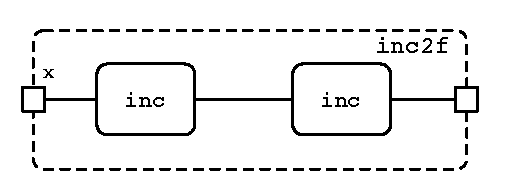
\includegraphics[height=2cm]{figs/inc2f}
  \caption{A representation of the \texttt{inc2f} wiring function defined in
    listing~\ref{lst:caph-ex14}}
  \label{fig:inc2f}
\end{figure}
 
\begin{figure}[h]
  \centering
  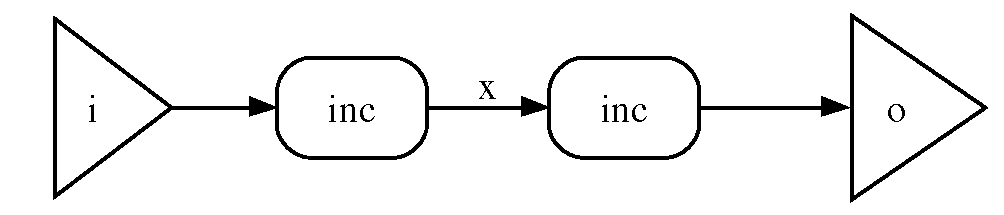
\includegraphics[height=1.5cm]{figs/smallnet2}
  \caption{The network resulting from applying the \texttt{inc2f} function}
  \label{fig:inc2fapp}
\end{figure}

\medskip
Wiring functions can take several arguments. In this case, arguments can be passed either as a tuple
or as a sequence.

\begin{lstlisting}[title=Example]
net foo (x,y) = add (x, inc y);
net o = foo (i1,i2);
\end{lstlisting}

The previous example could also have been written (strictly equivalent form)~: 

\begin{lstlisting}
net foo x y = add (x, inc y);
net o = foo i1 i2;
\end{lstlisting}

When this second definition form for the \texttt{foo} function\footnote{Technically known as the
  \emph{curried} form.} is used as above, it is strictly equivalent to the first one (in other
words, the network corresponding to the two previous programs are identical). But the second form
has a bonus~: it allows \emph{partial application} of the \texttt{foo} function. Partial application
means fixing the value of some arguments to obtain another function, which can be viewed as
``specialized'' version of the original one. In our case, partial application means fixing some part
of the sub-network defined by the original function.
For example, if we write

\begin{lstlisting}
net foo1 = foo i;
\end{lstlisting}

then \texttt{foo1} is the function obtained by assigning the value \texttt{i} to \texttt{x} in the
definition of \texttt{foo} (Fig.~\ref{fig:addinc}). In other words, the
\texttt{foo1} function is equivalent to the function that could have been written as

\begin{lstlisting}
net foo2 y = add (i, inc y);
\end{lstlisting}


\begin{figure}[h]
\begin{tabular}[c]{cc}
\begin{minipage}[b]{0.5\linewidth}
\begin{center}
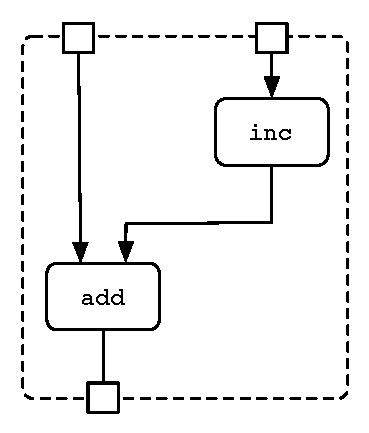
\includegraphics[width=0.5\linewidth]{figs/addinc}
%\caption{\texttt{net foo = add (x, inc y)}}
%\label{fig:addinc1}
\end{center}
\end{minipage}
&
\begin{minipage}[b]{0.5\linewidth}
\begin{center}
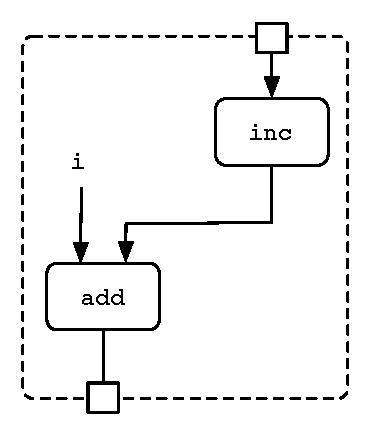
\includegraphics[width=0.5\linewidth]{figs/addinc2}
%\caption{\texttt{net foo1 = foo i}}
%\label{fig:addinc2}
\end{center}
\end{minipage} \\
\texttt{net foo = add (x, inc y);} &
\texttt{net foo1 = foo i;}
\end{tabular}
\caption{Partial application}
\label{fig:addinc}
\end{figure}

Then, the three programs of Fig.~\ref{fig:threepgms} are stricly equivalent~:

\begin{figure}[h]
\begin{tabular}[c]{ccc}
  \begin{minipage}[b]{0.33\linewidth}
    \begin{lstlisting}
    net foo x y =
      add (x, inc y);
    net o = foo i1 i2;
    \end{lstlisting} 
  \end{minipage} &
  \begin{minipage}[b]{0.33\linewidth}
    \begin{lstlisting}
    net foo x y =
       add (x, inc y);
    net foo1 = foo i1;
    net o = foo1 i2;
    \end{lstlisting} 
  \end{minipage} &
  \begin{minipage}[b]{0.33\linewidth}
    \begin{lstlisting}
    net foo2 y =
      add (i1, inc y);
    net o = foo2 i2;
    \end{lstlisting} 
  \end{minipage}
\end{tabular}
  \caption{Three equivalent programs}
  \label{fig:threepgms}
\end{figure}

\medskip
\textbf{Higher-order wiring functions}. For now we have been passing only \emph{wires} as arguments to
wiring functions. But functions can also be passed as arguments to wiring functions

\begin{lstlisting}[title=Example]
net twice (f,x) = f (f x);
\end{lstlisting}

The \texttt{twice} (higher-order) function takes two arguments, a function \texttt{f} and a wire
\texttt{x}. It instanciates the sub-network corresponding to \texttt{f} a first time, binding its
input to the \texttt{x} wire, and then a second time, binding the former output to the input of the
latter. For example, writing~:

\begin{lstlisting}
net o = twice (inc2f,i);
\end{lstlisting}

produces the network depicted in Fig.~\ref{fig:twice}.

\begin{figure}[h]
  \centering
  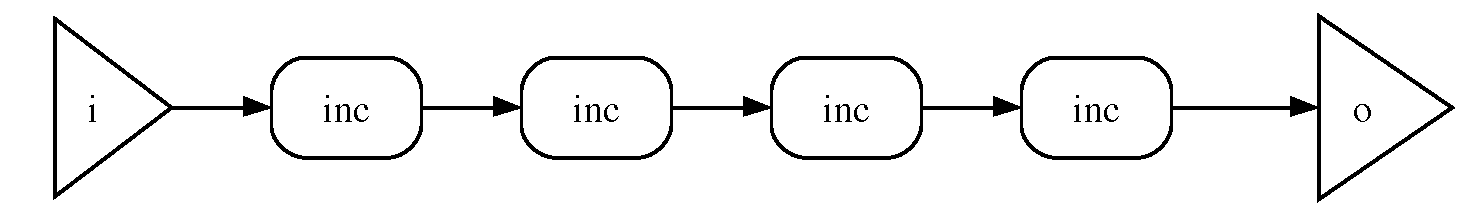
\includegraphics[height=1.5cm]{figs/twice}
  \caption{\texttt{net o = twice (inc2f, i)}}
  \label{fig:twice}
\end{figure}

\medskip
This is the combination of partial application and higher-order functions that
allows the encapsulation of graph patterns as wiring functions, as illustrated in
Sec.~\ref{sec:network-lang} with the function \texttt{diamond}. In the last example of this Section
: 

\begin{lstlisting}
net o = diamond (dup, inc, diamond (dup,inc,dec,mul), mul) i;
\end{lstlisting}

the inner application of function \texttt{diamond} is partial, so that it can be passed, as a wiring
function, as an argument to the outer application.

\subsubsection{Recursive wiring}
\label{sec:recursive-wiring}

By recursive wiring, we mean the ability for a box (resp. set of boxes) to take as input some wires
originating, directly or indirectly, from its (resp. their) output(s).

This is illustrated in Fig.~\ref{fig:rec-ex1}, where the network on the left is described by the
program on the right. Here, the second output of actor \texttt{A} is
re-injected, after passing through actor \texttt{B} to its second input.

\begin{figure}[h]
  \centering
  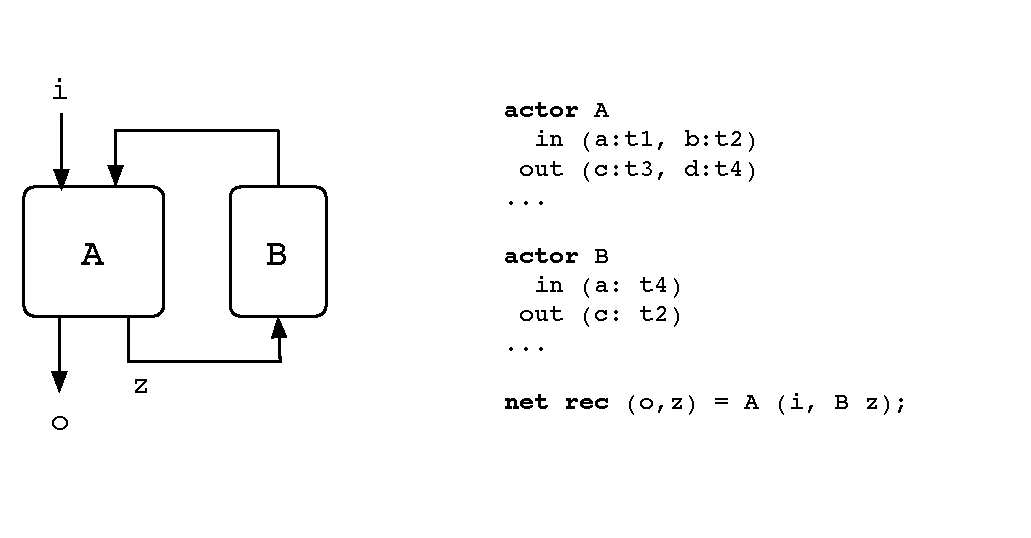
\includegraphics[width=0.75\textwidth]{figs/rec1}
  \caption{Example of recursive wiring}
  \label{fig:rec-ex1}�
\end{figure}

Mutually recursive wiring between actors is also possible, as shown on Fig.~\ref{fig:rec-ex2}.

\begin{figure}[h]
  \centering
  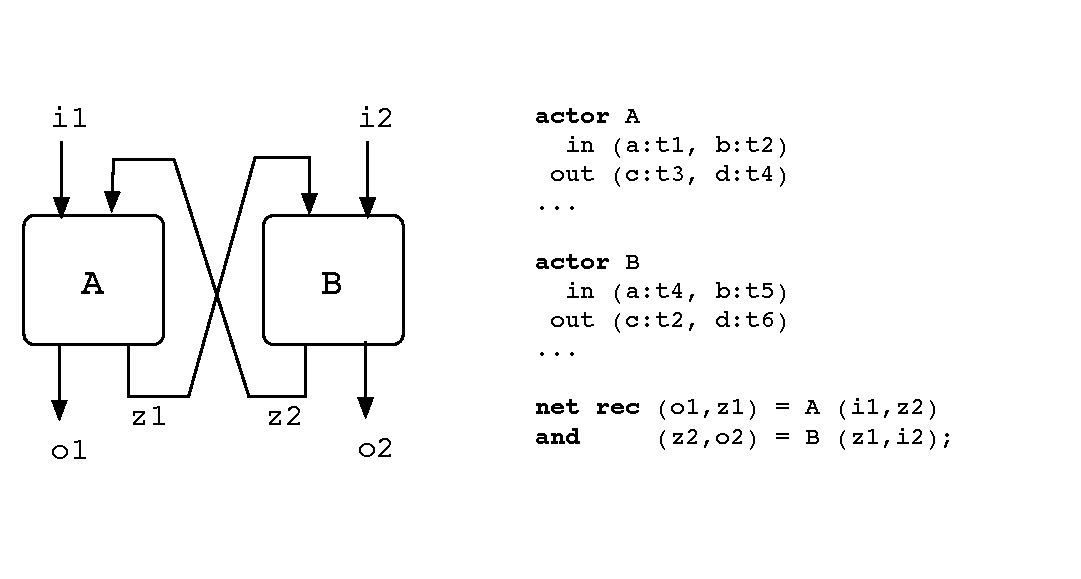
\includegraphics[width=0.75\textwidth]{figs/rec2}
  \caption{Example of mutually recursive wiring}
  \label{fig:rec-ex2}
\end{figure}
 
\medskip As shown above, recursive wiring is used to describe \emph{cyclic} networks.  In the
classical dataflow model, cycles are typically used to implement iterations~\cite{Davis82}.  In
\caph, iterations are generally handled at the actor level, using local variables.

Functionnaly, the two formulations are equivalent~:  in the recursive version,
the ``state'' memorized in the local variables is simply ``externalized'' and held in the looping
wires. 

To illustrate this, let's go back to the actor \texttt{suml} introduced at the end of
section~\ref{sec:actor-examples}~:

\begin{lstlisting}[caption=\relax,label=lst:caph-ex15]
actor suml
  in (i:signed<16> dc)
  out (o:signed<16>)
var state : { S0, S1 } = S0
var sum : int
rules 
  | (state:S0, i:'<) -> (sum:0, state:S1)
  | (state:S1, i:'>) -> (o:sum, state:S0)
  | (state:S1, i:'v) -> (sum:sum+v);
\end{lstlisting}

The \texttt{suml} actor computes the sum of each list given as input, using two local variables : one holding the
state of the computation and the other the accumulator. This actor can be used, for example, in the
following program~:

\begin{lstlisting}[caption=\relax,label=lst:caph-ex16]
actor suml  ... -- as above

stream i:signed<16> dc from "sample.txt";
stream o:signed<16> to "result.txt";

net o = suml i;
\end{lstlisting}

If the input file \texttt{sample.txt} contains, let say

\begin{center}
\begin{verbatim}
< 1 2 3 > < 4 5 6 >
\end{verbatim}
\end{center}

then output file \texttt{result.txt} will contain 

\begin{center}
\begin{verbatim}
6 15
\end{verbatim}
\end{center}

Listing~\ref{lst:caph-ex17} shows an equivalent program based on a variant of the \texttt{suml} actor in which
local variables have been replaced by feedback wires~:

\begin{lstlisting}[caption=A recursive reformulation of actor \texttt{suml},label=lst:caph-ex17]
actor suml_rec 
  in (i:signed<16> dc, sum:signed<16>)
 out (o:signed<16>, nsum:signed<16>)
rules
| (i:'<       ) -> nsum:0
| (i:'>, sum:s) -> o:s
| (i:'v, sum:s) -> nsum:s+v
;

stream i : signed<16> dc from "sample.txt";
stream o : signed<16> to "result.txt";

net rec (o,z) = suml_rec (i,z);
\end{lstlisting}

Note that \texttt{suml\_rec} is a \emph{state-less} actor~: it has no local variable. The running
sum is now implicitely kept on a external feedback wire, connecting its \texttt{nsum} output to its
\texttt{sum} input.  The three rules describing its behavior can be read as~:
\begin{itemize}
\item when reading a ``\verb|<|'' control token on input \texttt{i}, write the initial value of the
  accumulator on the feedback wire,
\item when reading a ``\verb|>|'' control token on input \texttt{i}, write the final value of the
  accumulator, available on input \texttt{sum}, on output \texttt{o},
\item when reading a value on both inputs, add these values and write the sum on the feedback wire.
\end{itemize}

\begin{figure}[h]
  \centering
  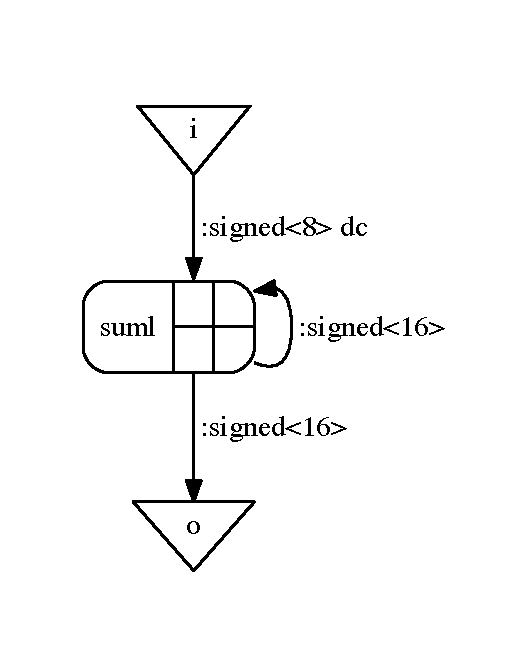
\includegraphics[height=8cm]{figs/suml-rec}
  \caption{A cyclic dataflow network}
  \label{fig:suml-rec}
\end{figure}

The corresponding dataflow graph is given in Fig.~\ref{fig:suml-rec}. 

Note that, if \emph{functionally} equivalent, this second program actually generates less efficient
code, since the recursive values must in this case pass through external links, which introduce
latencies. For this reason, formulations using local variables should always be prefered, when
possible, when writing \caph programs\footnote{There's a noticeable exception to this rule; it
  concerns the \texttt{d1lr} actor defined in library \texttt{img\_ops.cph} and implementing line delay on
  images. In this case, recursive wiring is deliberately used in order to have the delayed line
  stored in a external FIFO, because this scheme is more efficiently handled by the VHDL
  synthetisers.}. 

\subsubsection{Higher-order wiring primitives}
\label{sec:bundles}

Just like certain kinds of actor behavior can be encapsulated using higher order actors (see
Sec.~\ref{sec:higher-order-actors}), certain patterns in data-flow graphs can be encoded concisely in \caph using 
so-called \emph{higher-order wiring primitives}. The four basic higher-order primitives are
\texttt{map}, \texttt{napp}, \texttt{foldl} and \texttt{pipe}.

\medskip
The \textbf{map} higher-order primitive\footnote{Not to be confused with the \texttt{smap} higher
  order \emph{actor}.} is illustrated in Fig.~\ref{fig:map-ex0}. It is used
whenever the same processing has to be carried out on a set of separate data streams.

\begin{figure}[h]
\centering
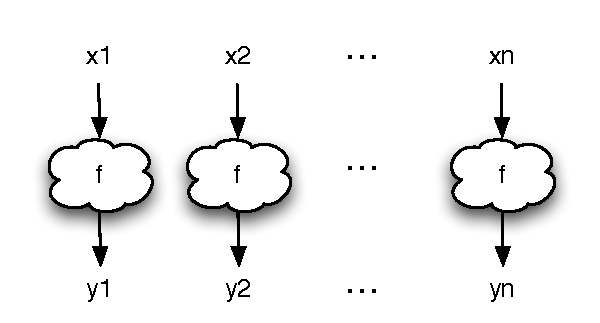
\includegraphics[width=0.7\textwidth]{figs/map-ex0.pdf}
\caption{A parallel graph pattern}
\label{fig:map-ex0}
\end{figure}

A simple description of the graph given in Fig.~\ref{fig:map-ex0} can be given by simply replicating
\texttt{net} definitions~:

\begin{lstlisting}
net y1 = f x1;
net y2 = f x2;
...
net yn = f xn;
\end{lstlisting}

The \verb|map| higher-order primitive offers a more concise way of describing this graph~:

\begin{lstlisting}
net (y1,y2,...,yn) = map f (x1,x2,...,xn);
\end{lstlisting}

The \texttt{map} function takes two arguments~:
\begin{itemize}
\item a wiring function $f$, with type $\tau \rightarrow \tau'$,
\item a tuple $(x_1,\ldots,x_n)$ of wires\footnote{Actually, and for technical reasons, the type of the second argument
    \texttt{map} is not $(\tau,\ldots,\tau)$ but $(\tau,\alpha)~\emtxt{bundle}$, where
    $\emtxt{bundle}$ is a built-in type constructor for representing bundles of homogeneous
    types. The type-checking phases unifies the types $\underbrace{(\tau,\ldots,\tau)}_{n}$ and
    $(\tau,n)~\emtxt{bundle}$. Since this unification is carried out automatically by the type
    checker, the \texttt{map} function can be viewed as operating and returning directly tuples of
    values (of the same type, of course).}, each having type $\tau$
\end{itemize}
and returns a tuple of wires, each of type $\tau'$, by applying the $f$ function to each wire $x_i$.
In other words~:

\begin{equation*}
  \text{map}\ f\ (x_1,\ldots,x_n) = (f\ x_1, \ldots, f\ x_n)
\end{equation*}

The first argument of \texttt{map} can be an simple actor, with or without parameter(s) or a complex
wiring function, as illustrated in Fig.~\ref{fig:map-ex1}, \ref{fig:map-ex2} and \ref{fig:map-ex3}. 

\begin{figure}[h!]
  \centering
  \begin{tabular}[t]{cc}
    \begin{minipage}[c]{0.5\linewidth}
      \begin{lstlisting}
actor double 
  in (a:unsigned<8>)
  out (c:unsigned<8>)
rules a -> c
| x -> 2*x
;

net i1 = ...
net i2 = ...

net (o1,o2) = map double (i1,i2);
      \end{lstlisting}
    \end{minipage}
\adjustbox{valign=c}{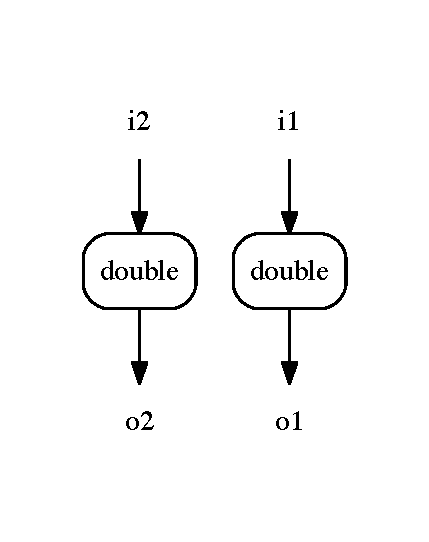
\includegraphics[width=0.4\linewidth]{figs/map-ex1}}
  \end{tabular}
  \caption{\texttt{map} - example 1}
  \label{fig:map-ex1}
\end{figure}

\begin{figure}[h!]
  \centering
  \begin{tabular}[t]{cc}
    \begin{minipage}[c]{0.5\linewidth}
      \begin{lstlisting}
actor scale (k:unsigned<8>) 
  in (a:unsigned<8>)
  out (c:unsigned<8>)
rules a -> c
| x -> 2*x
;

net i1 = ...
net i2 = ...

net (o1,o2) = map (scale 2) (i1,i2);
      \end{lstlisting}
    \end{minipage}
\adjustbox{valign=c}{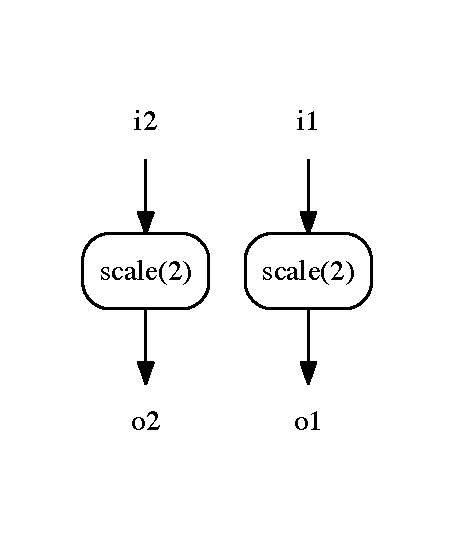
\includegraphics[width=0.4\linewidth]{figs/map-ex2}}
  \end{tabular}
  \caption{\texttt{map} - example 2}
  \label{fig:map-ex2}
\end{figure}

\begin{figure}[h!]
  \centering
  \begin{tabular}[t]{cc}
    \begin{minipage}[c]{0.5\linewidth}
      \begin{lstlisting}
actor scale (k:unsigned<8>) 
  in (a:unsigned<8>)
  out (c:unsigned<8>)
rules a -> c
| x -> 2*x
;

net i1 = ...
net i2 = ...

net f x = scale 2 (scale 4 x);

net (o1,o2) = map f (i1,i2);
      \end{lstlisting}
    \end{minipage}
\adjustbox{valign=c}{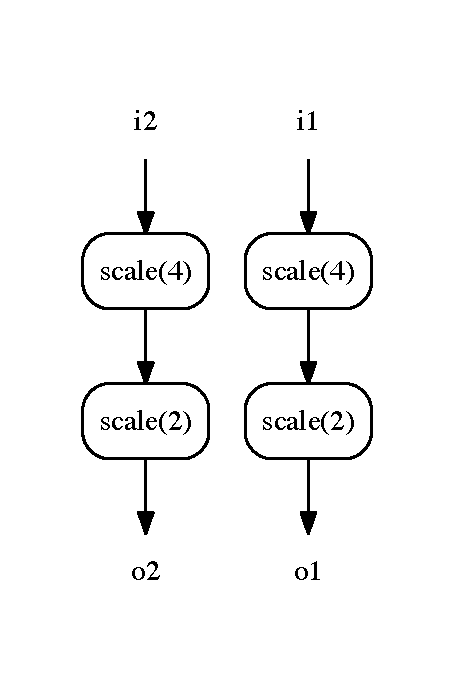
\includegraphics[width=0.35\linewidth]{figs/map-ex3}}
  \end{tabular}
  \caption{\texttt{map} - example 3}
  \label{fig:map-ex3}
\end{figure}
 

\medskip A very useful variant of the \texttt{map} function is \texttt{mapi}.  As \texttt{map}, the
\texttt{mapi} function takes two arguments, a wiring function $f$, with type $\text{unsigned} \rightarrow
\tau \rightarrow \tau'$ and a tuple of wires, and returns a tuple of wires, obtained by applying the $f$ function to
each wire of the input tuple. But the $f$ function here takes an extra argument which is
automatically set to the index\footnote{Starting at 0, not 1.} of the corresponding wire in the
input tuple.  In other words, and more precisely~:

\begin{equation*}
  \text{mapi}\ f\ (x_1,\ldots,x_n) = (f\ 0\ x_1, \ldots, f\ (n-1)\ x_n)
\end{equation*}

A typical usage of the \texttt{mapi} function is given in Fig~\ref{fig:mapi-ex1}.  Here the extra
argument (ranging from 0 to 3) is used to adjust the scaling factor applied in each branch of the
parallel pattern.

As for the \texttt{map} function, the first argument of the \texttt{mapi} function can be an
actor or a any wiring function having a type of the form $\text{unsigned} \rightarrow \tau' \rightarrow
\tau'$~:

\begin{figure}[h!]
  \centering
  \begin{tabular}[t]{cc}
    \begin{minipage}[c]{0.6\linewidth}
\small
      \begin{lstlisting}
const coeff = [2,4,8,16] : unsigned<8> array[4];

actor scale (k:unsigned<8>) 
  in (a:unsigned<8>)
  out (c:unsigned<8>)
rules a -> c
| x -> k*x
;

net i1 = ...
net i2 = ...
net i3 = ...
net i4 = ...

net f i x = scale (coeff[i]) x;

net (o1,o2,o3,o4) = mapi f (i1,i2,i3,i4);
      \end{lstlisting}
\normalsize
    \end{minipage}
\adjustbox{valign=c}{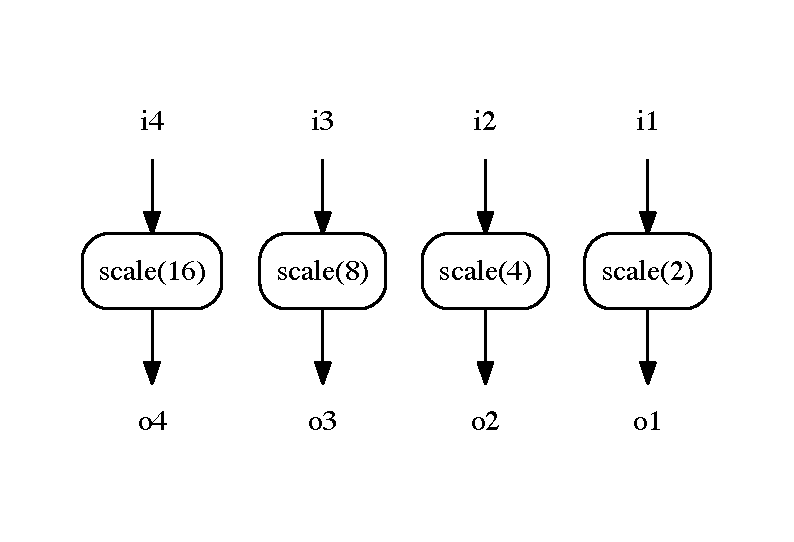
\includegraphics[width=0.4\linewidth]{figs/mapi-ex1}}
  \end{tabular}
  \caption{\texttt{mapi} - example}
  \label{fig:mapi-ex1}
\end{figure}

\medskip Another variant of the \texttt{map} function is \texttt{map2}. 
The \texttt{map2} function takes three arguments~:
\begin{itemize}
\item a wiring function $f$, with type $\tau_1 \times \tau_2 \rightarrow \tau'$,
\item a first tuple of wires, each with type $\tau_1$,
\item a second tuple of wires, each with type $\tau_2$,
\end{itemize}
and returns a tuple of wires, obtained by applying the $f$ function to each pair of input wires.
In other words~:

\begin{equation*}
  \text{map2}\ f\ ((x_1,\ldots,x_n),(y_1,\ldots,y_n)) = (f\ (x_1,y_1), \ldots, f\ (x_n,y_n))
\end{equation*}

Of course, the two input tuples must have the same size. Fig.~\ref{fig:map2-ex1} gives an example involving the
\texttt{map2} function.

\begin{figure}[h!]
  \centering
  \begin{tabular}[t]{cc}
    \begin{minipage}[c]{0.5\linewidth}
\small
      \begin{lstlisting}
actor add (k:unsigned<8>)
  in (a:unsigned<8>, b:unsigned<8>)
  out (c:unsigned<8>)
rules (a,b) -> c
| (x,y) -> k*x+y
;

net i11 = ...
net i12 = ...
net i21 = ...
net i22 = ...

net (o1,o2) =
  map2 (add 2) ((i11,i12),(i21,i22));
      \end{lstlisting}
\normalsize
    \end{minipage}
\adjustbox{valign=c}{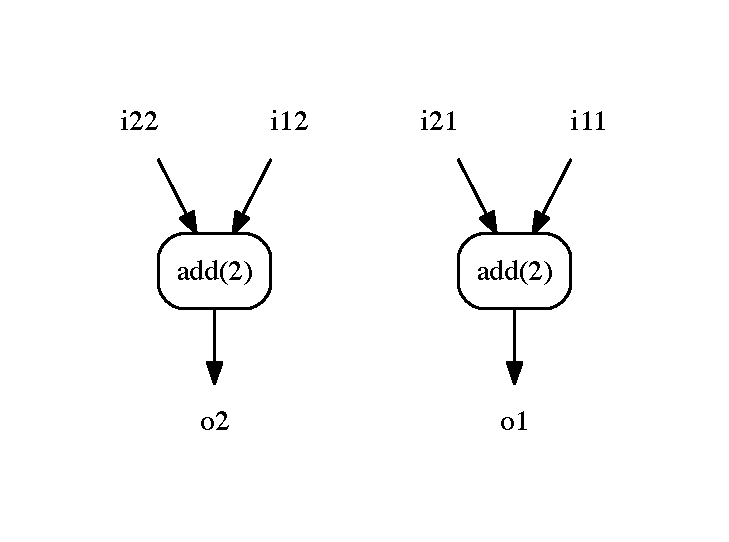
\includegraphics[width=0.5\linewidth]{figs/map2-ex1}}
  \end{tabular}
  \caption{\texttt{map2} - example}
  \label{fig:map2-ex1}
\end{figure}

\medskip As for the \texttt{map} function, \texttt{map2} has a variant, named \texttt{map2i} for
which the function argument takes an extra argument~:

\begin{equation*}
  \text{map2i}\ f\ ((x_1,\ldots,x_n),(y_1,\ldots,y_n)) = (f\ 0\ (x_1,y_1), \ldots, f\ (n-1)\
  (x_n,y_n))
\end{equation*}

\bigskip
With the \texttt{map} family of higher-order primitives, the same processing is replicated over a
set of distinct data streams (the number of streams giving the ``width'' of the data-flow
graph). The \texttt{napp} higher-order primitive offers a way of replicating a processing on the
\emph{same} data stream, the number of replications (the ``width'' of the graph) being here
specified as an extra argument. Typical examples are given in Fig.~\ref{fig:napp-ex1} and
\ref{fig:napp-ex2}. 

The \texttt{napp} function takes three arguments~:
\begin{itemize}
\item a integer $n$ (which must be a statically bound constant),
\item a wiring function $f$, with type $\tau \rightarrow \tau'$,
\item a wire $x$, of type $\tau$
\end{itemize}
and returns a tuple of $n$ wires, each of type $\tau'$, by applying $n$ times the $f$ function to wire $x$.
In other words~:

\begin{equation*}
  \text{napp}\ n\ f\ x = (\underbrace{f\ x, \ldots, f\ x}_{n})
\end{equation*}

As for \texttt{map}, \texttt{nappi} is a variant of \texttt{napp} for which the applied fonction
($f$) takes a extra parameter automatically bound to the replication index :

\begin{equation*}
  \text{nappi}\ n\ f\ x = (f\ 0\ x, \ldots, f\ (n-1)\ x)
\end{equation*}

The \texttt{nappi} higher-order primitive is illustrated in Fig.~\ref{fig:nappi-ex1} (with $n=3$).

\begin{figure}[h!]
  \centering
  \begin{tabular}[t]{cc}
    \begin{minipage}[c]{0.5\linewidth}
      \begin{lstlisting}
actor double 
  in (i:unsigned<8>)
  out (o:unsigned<8>)
rules 
| i:x -> o:2*x
;

stream i:unsigned<8> ...
stream o1:unsigned<8> ...
stream o2:unsigned<8> ...
stream o3:unsigned<8> ...

net (o1,o2,o3) = napp 3 double i;
      \end{lstlisting}
    \end{minipage}
\adjustbox{valign=c}{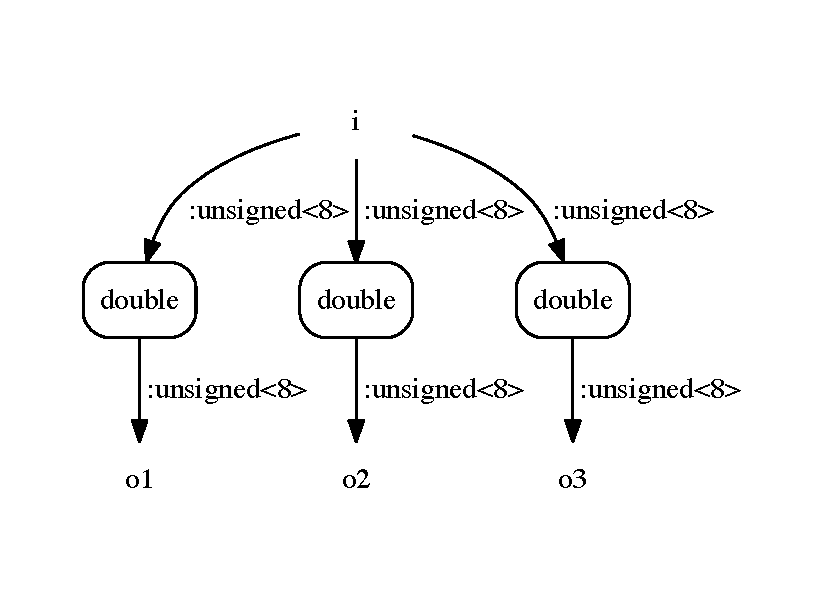
\includegraphics[width=0.4\linewidth]{figs/napp-ex1}}
  \end{tabular}
  \caption{\texttt{napp} - example 1}
  \label{fig:napp-ex1}
\end{figure}

\begin{figure}[h!]
  \centering
  \begin{tabular}[t]{cc}
    \begin{minipage}[c]{0.5\linewidth}
      \begin{lstlisting}
actor addm
  in (i1:unsigned<8>, i2:unsigned<8>)
  out (o:unsigned<8>)
rules 
| (i1:x1, i2:x2) -> o:x1+x2
;

stream i1:unsigned<8> ...
stream i2:unsigned<8> ...
stream o1:unsigned<8> ...
stream o2:unsigned<8> ...

net (o1,o2) = napp 2 addm (i1,i2);
      \end{lstlisting}
    \end{minipage}
\adjustbox{valign=c}{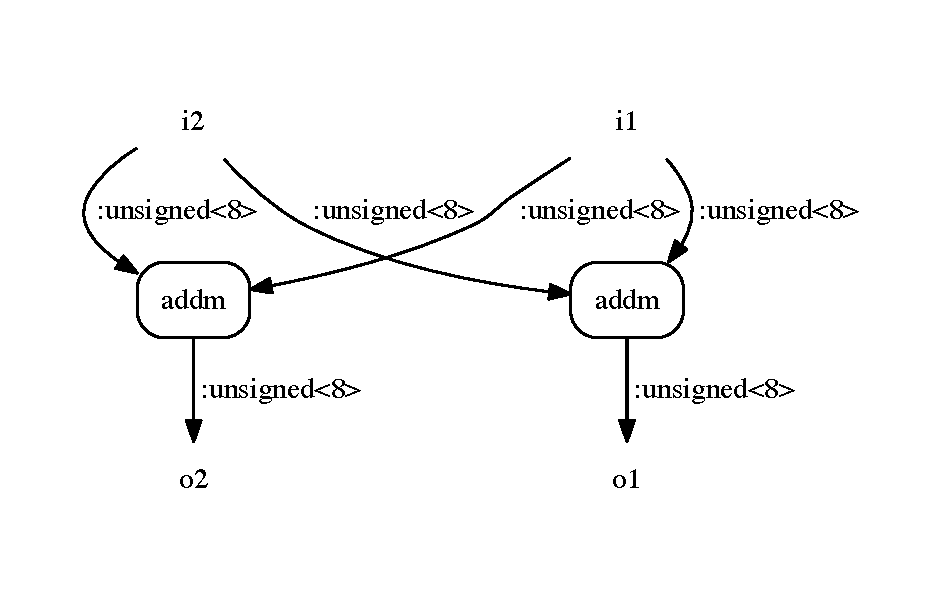
\includegraphics[width=0.4\linewidth]{figs/napp-ex2}}
  \end{tabular}
  \caption{\texttt{napp} - example 2}
  \label{fig:napp-ex2}
\end{figure}

\begin{figure}[h!]
  \centering
  \begin{tabular}[t]{cc}
    \begin{minipage}[c]{0.5\linewidth}
      \begin{lstlisting}
actor scale (k: unsigned<8>) 
  in (i:unsigned<8>)
  out (o:unsigned<8>)
rules 
| i:x -> o:(k+1)*x
;

stream i:unsigned<8> ...
stream o1:unsigned<8> ...
stream o2:unsigned<8> ...
stream o3:unsigned<8> ...

net (o1,o2,o3) = nappi 3 scale i;
      \end{lstlisting}
    \end{minipage}
\adjustbox{valign=c}{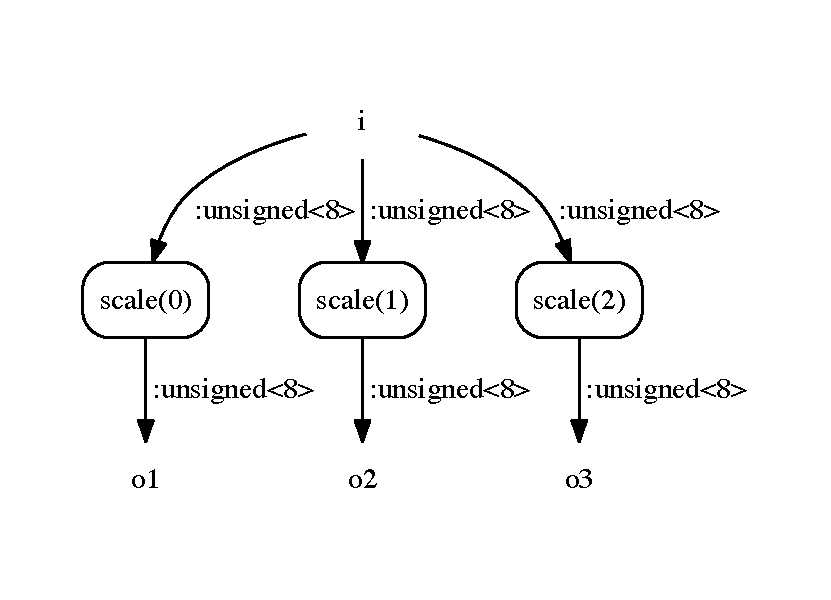
\includegraphics[width=0.4\linewidth]{figs/nappi-ex1}}
  \end{tabular}
  \caption{\texttt{nappi} - example}
  \label{fig:nappi-ex1}
\end{figure}


\bigskip The \texttt{map} function (and its variants \texttt{mapi}, \texttt{map2} and
\texttt{map2i}) encodes parallel \emph{replication} graph patterns. Another higher-order wiring
primitive, \texttt{foldl} (fold left)\footnote{Not to be confused with the \texttt{sfold} and
  \texttt{ssfold} higher order \emph{actors}.} is provided for encoding parallel \emph{reduction} patterns.
Formally, if $x=(x_1,\ldots,x_n)$ is a tuple of values having type $\tau$ and $f$ a function having
type $\tau \times \tau \rightarrow \tau$, then 
\begin{equation*}
  \text{foldl}\ f\ (x_1,\ldots,x_n) = f (\ldots f(f(x_1,x_2),x_3)\ldots, x_n)
\end{equation*}
In other words, the result of applying \emph{foldl} to $f$ and $x$ is obtained by applying $f$ as a
binary reduction operator over the tuple $x$.
An example showing the effect of the \texttt{foldl} function is given in Fig.~\ref{fig:foldl-ex1}. 

\begin{figure}[h!]
  \centering
  \begin{tabular}[t]{cc}
    \begin{minipage}[c]{0.5\linewidth}
      \begin{lstlisting}
actor madd (k: unsigned<8>)
  in (a:unsigned<8>, b:unsigned<8>)
  out (c:unsigned<8>)
rules (a,b) -> c
| (x,y) -> x*k+y
;

net i1 = ...
net i2 = ...
net i3 = ...
net i4 = ...

net f (x,y) = madd 2 (x,y);

net o = foldl f (i1,i2,i3,i4);
      \end{lstlisting}
    \end{minipage}
\adjustbox{valign=c}{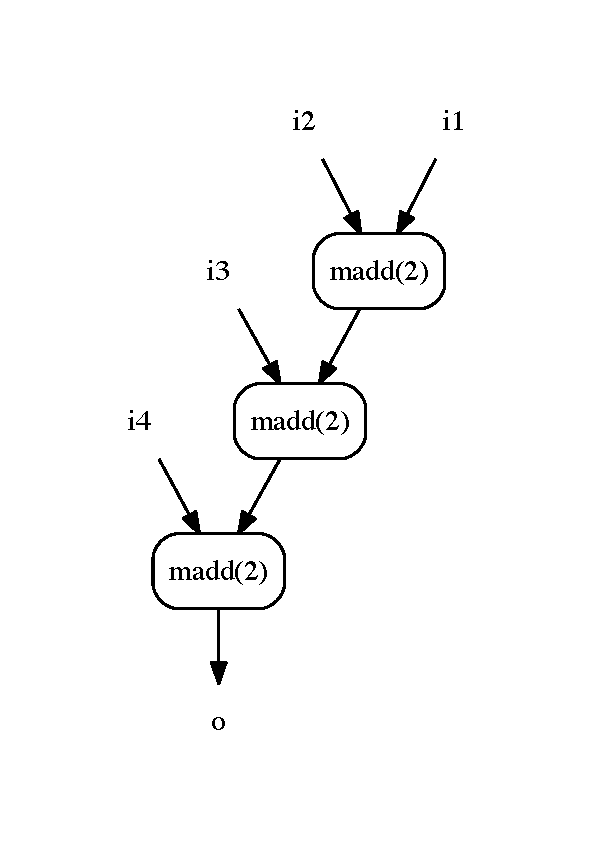
\includegraphics[width=0.4\linewidth]{figs/foldl-ex1}}
  \end{tabular}
  \caption{\texttt{foldl} - example}
  \label{fig:foldl-ex1}
\end{figure}

\medskip As for \texttt{map}, the \texttt{foldl} function has a variant, named \texttt{foldli} for dealing with
\emph{indexed} reduction.
Formally, if $x=(x_1,\ldots,x_n)$ is a tuple of values having type $\tau$ and $f$ a function having
type $\text{unsigned} \rightarrow \tau \times \tau \rightarrow \tau$, then 
\begin{equation*}
  \text{foldli}\ f\ ((x_1,\ldots,x_n) = f\ (n-1)\ (\ldots f\ 1\ (f\ 0\ (x_1,x_2),x_3)\ldots, x_n)
\end{equation*}

\medskip A last variant of the \texttt{foldl} function is \texttt{foldt}, which performs a
\emph{dyadic} reduction, as shown in Fig.~\ref{fig:foldt-ex}.

\begin{figure}[h!]
  \centering
  \begin{tabular}[t]{cc}
    \begin{minipage}[c]{0.5\linewidth}
      \begin{lstlisting}
actor add 
  in (a:unsigned<8>, b:unsigned<8>)
  out (c:unsigned<8>)
rules (a,b) -> c
| (x,y) -> x+y;

net i1 = ...
net i2 = ...
net i3 = ...
net i4 = ...

net o = foldt add (i1,i2,i3,i4);
      \end{lstlisting}
    \end{minipage}
\adjustbox{valign=c}{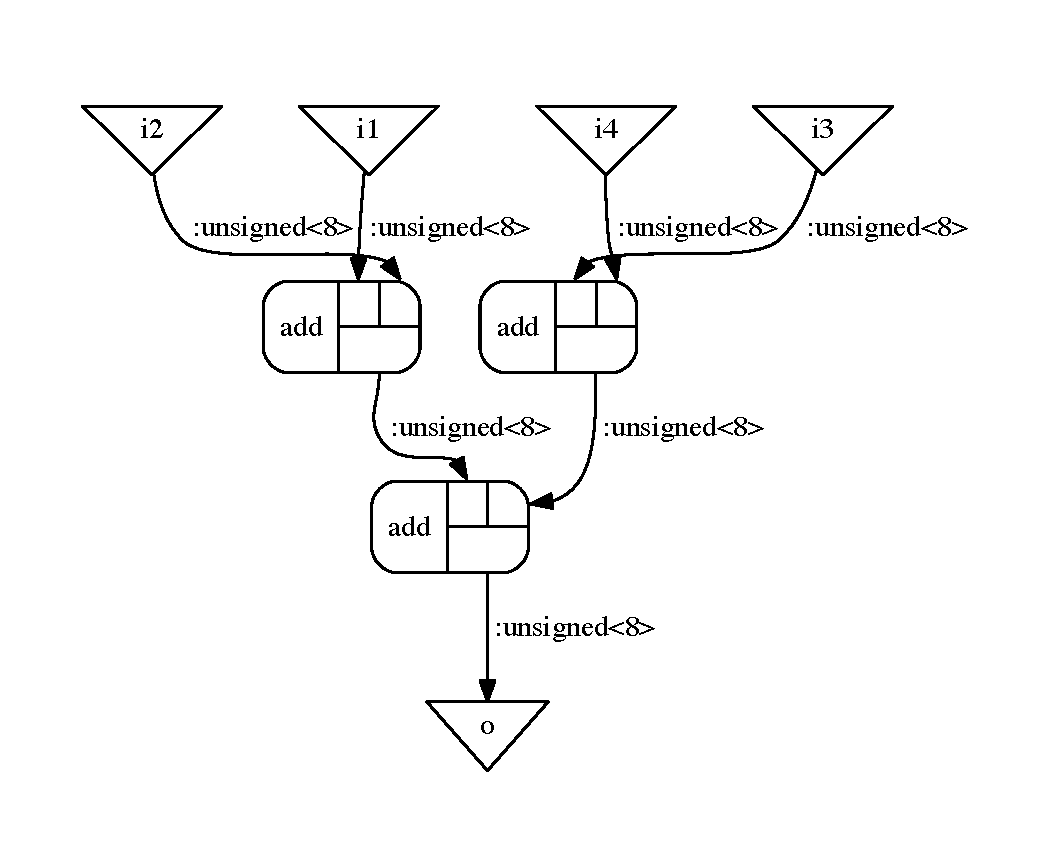
\includegraphics[width=0.4\linewidth]{figs/foldt-ex}}
  \end{tabular}
  \caption{\texttt{foldt} - example}
  \label{fig:foldt-ex}
\end{figure}

\bigskip The \texttt{pipe} higher-order wiring primitive can be used to encode linear ``pipelined''
graph patterns, as illustrated in Fig.~\ref{fig:pipe-ex}.

\begin{figure}[h!]
  \centering
  \begin{tabular}[t]{cc}
    \begin{minipage}[c]{0.5\linewidth}
      \begin{lstlisting}
actor double 
  in (a:unsigned<8>)
  out (c:unsigned<8>)
rules a -> c
| x -> 2*x ;

net i = ...

net o = pipe 4 double i;
      \end{lstlisting}
    \end{minipage}
\adjustbox{valign=c}{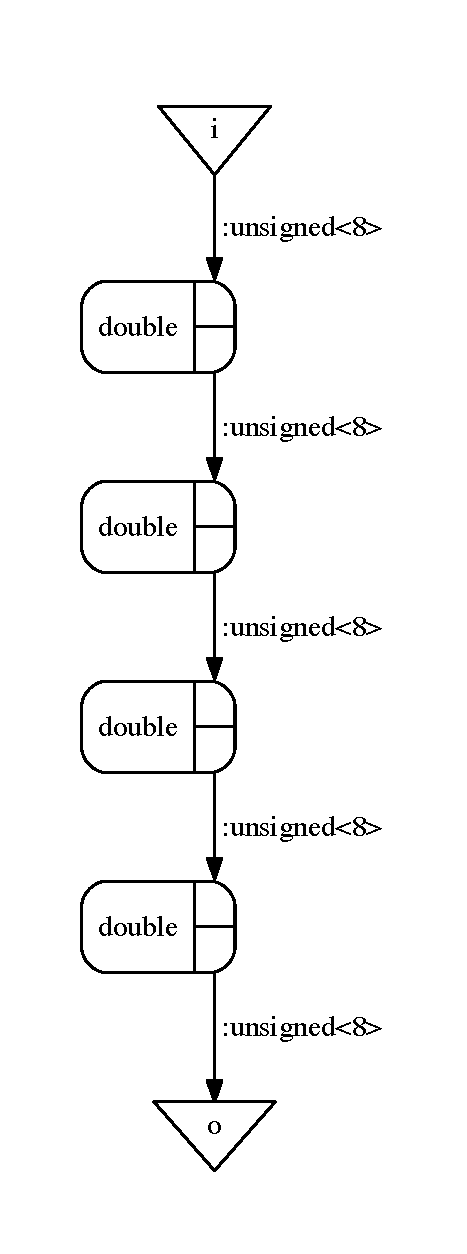
\includegraphics[width=0.2\linewidth]{figs/pipe-ex}}
  \end{tabular}
  \caption{\texttt{pipe} - example}
  \label{fig:pipe-ex}
\end{figure}

\section{A complete example}
\label{sec:complete-example}

Listing~\ref{lst:grad-ex} gives the full \caph source code of a basic application for extracting
edges in images. Figure~\ref{fig:grad-net} gives the corresponding dataflow network.

For each pixel $P_{i,j}$, the local gradient magnitude is approximated by the sum of the absolute
value of the horizontal and vertical derivatives ($|P_{i,j}-P_{i,j-1}|+|P_{i,j}-P_{i-1,j}|$) and the
resulting value is compared to a fixed threshold for producing a binary image (with edge pixels
encoded as 1 and background pixels as 0).

An example of input and output image (obtained with the simulator) is given Fig.~\ref{fig:lena-ex}.

\begin{figure}[h]
\centering
  \begin{tabular}[c]{cc}
  
\includegraphics[width=3cm]{figs/lena128.pdf} &
  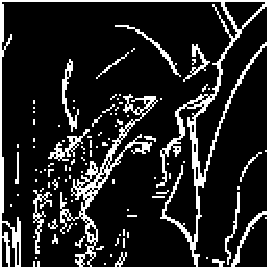
\includegraphics[width=3cm]{figs/lena128-grad.pdf} \\
  Input image & Result image
  \end{tabular}
  \caption{}
  \label{fig:lena-ex}
\end{figure}


Five actors are involved in this application~:
\begin{itemize}
\item the \texttt{d1p} and \texttt{d1l} actors are defined in the library \verb|img_ops.cph|\footnote{See
    chap.~\ref{cha:stdlib}; \texttt{d1l} is actually a wiring function invoking the \texttt{d1lr}
    actor in a recursive manner, as shown in Fig.~\ref{fig:grad-net}.}.  They are used by the
  \texttt{dx} and \texttt{dy} wiring functions (lines 31-32) to compute the horizontal and vertical
  derivatives. They delay an image by one pixel and by one line respectively, inserting a null value
  in the first colum (resp. line) and discarding the first column (resp. line). For example,
\small
  \begin{itemize}
  \item \verb|d1p:< < 1 2 3 4 > < 5 6 7 8 > > = < < 0 1 2 3 > < 0 5 6 7 > >|
  \item \verb|d1l:< < 1 2 3 4 > < 5 6 7 8 > > = < < 0 0 0 0 > < 0 1 2 3 > >|
  \end{itemize}
\normalsize
\item the \texttt{add} actor (lines 4-10) performs the normalized addition of two structured
  streams, preserving the structure; the \texttt{n} parameter is the normalization factor;
\item the \texttt{asub} actor (lines 13-19) computes the absolute value of the difference of two structured
  streams; for this it uses a global function \texttt{f\_abs} defined lines 1-2 of the program;
\item the \texttt{thr} actor (lines 22-28) binarizes a structured stream according to a given threshold; the
  threshold is specified as a parameter; the resulting stream contains only 0's and 1's.
\end{itemize}

Lines 31-32 defines the two wiring functions \texttt{dx} and \texttt{dy} computing the horizontal
and vertical derivatives of their argument. The \verb|[0]| argument passed to the \texttt{d1p} and
\texttt{d1l} actors is the value of the pixel inserted in the first column (resp. line).

For simulation and SystemC execution, the input (resp. output) stream is here read (written)
directly in (resp. to) a PGM file (this is an image) (lines 34-35). The input file will be specified
at compile time using the macro mechanism described in Sec~\ref{cha:using-caph-compiler}. 

Lines 37-38 gives the network description. The value \texttt{gm} is the image of the gradient magnitude (computed as
the sum of the absolute values of the horizontal and vertical derivatives). The result is obtained
by passing this image to the \texttt{thr} actor. As for the input file, the threshold value will be
specified here at compile time\footnote{A more adaptative approach would of course \emph{compute} this threshold
  from some statistics extracted from the input image.}.

\begin{lstlisting}[language=Caph,frame=single,numbers=left,caption={A basic edge extraction
    application in Caph},label={lst:grad-ex}]
function f_abs x =
  if x < 0 then -x else x : signed<m> -> signed<m>;

actor add (n:unsigned<4>)
  in (a:signed<m> dc, b:signed<m> dc)
  out (c:signed<m> dc)
rules (a,b) -> c
| ('<,'<) -> '<
| ('>,'>) -> '>
| ('p1,'p2) -> '(p1+p2)>>n ;

actor asub
  in (a:signed<m> dc, b:signed<m> dc)
  out (c:signed<m> dc)
rules (a,b) -> c
| ('<,'<) -> '<
| ('>,'>) -> '>
| ('p1,'p2) -> 'f_abs(p1-p2) ;

actor thr (t:signed<m>)
  in (a:signed<m> dc)
  out (c:unsigned<1> dc)
rules a -> c
| '< -> '<
| '> -> '>
| 'p -> if p > t then '1 else '0 ;

net dx i = asub (i, d1p 0 i);
net dy i = asub (i, d1l 0 i);

stream inp:signed<10> dc from "%arg1";
stream res:unsigned<1> dc to "result.txt";

net gm = add 0 (dx inp, dy inp);
net res = thr %arg2 gm;
\end{lstlisting}

\begin{figure}[h]
  \centering
  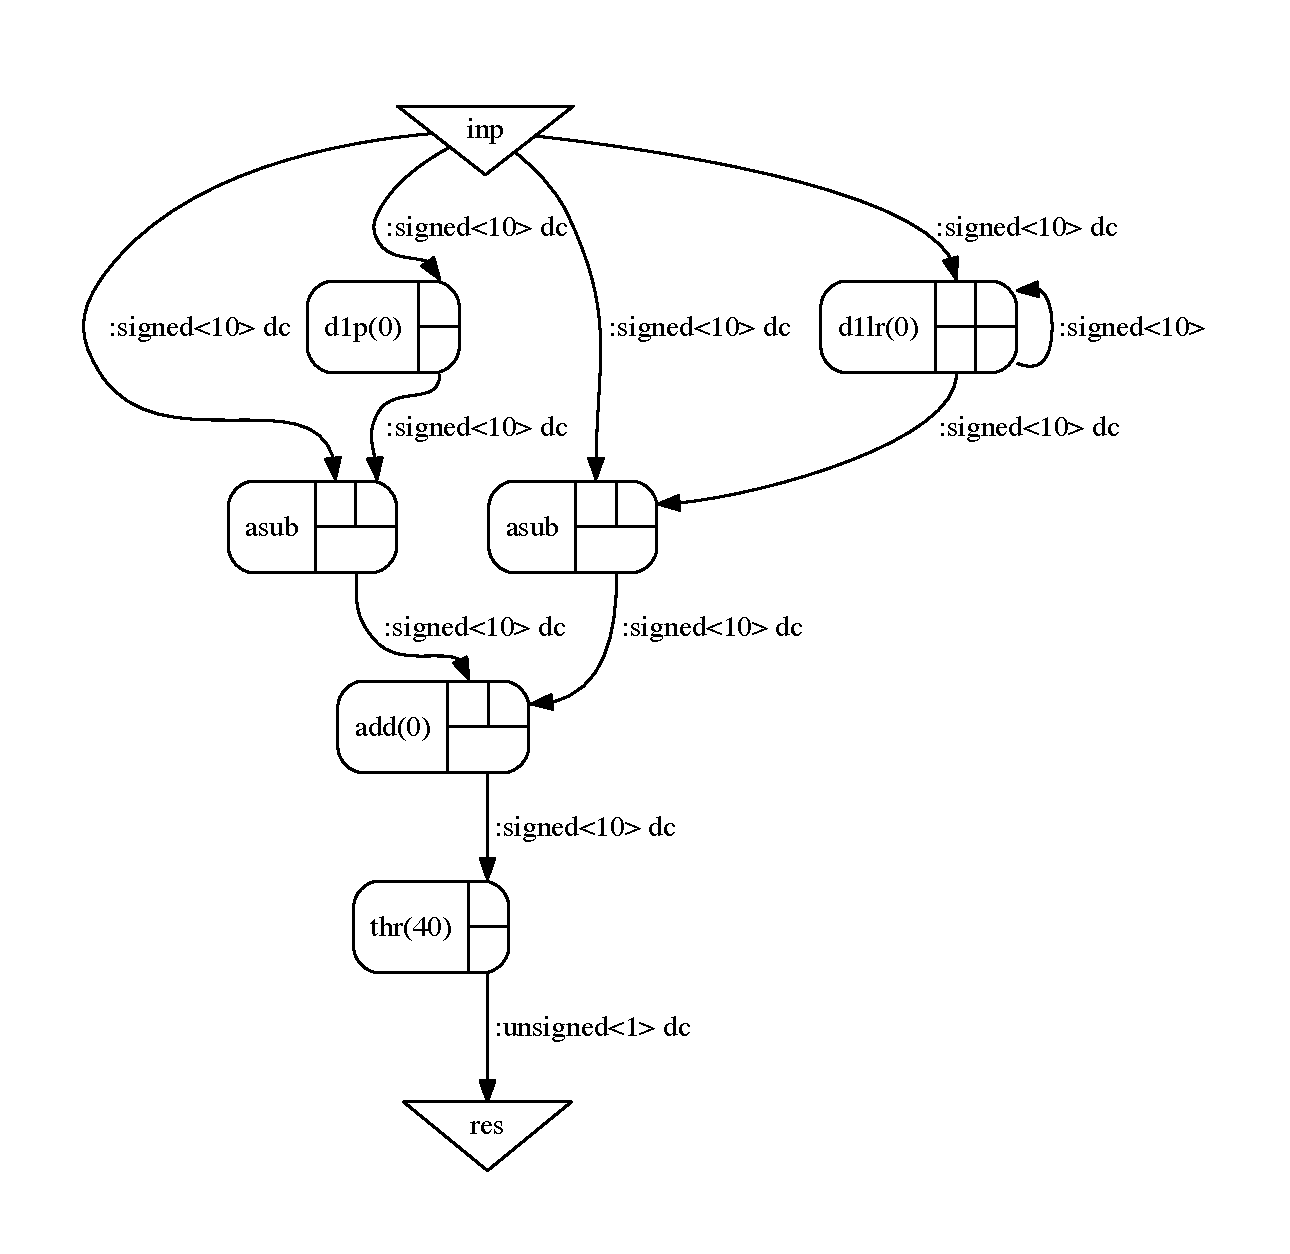
\includegraphics[width=0.90\textwidth]{figs/grad-net}
  \caption{The data-flow graph for the edge extraction application}
  \label{fig:grad-net}
\end{figure}

\medskip 
\noindent
\textbf{Note (version 2.8)}. The program given in listing~\ref{lst:grad-ex} can be rewritten in a
more concise manner using \emph{higher order actors} (see Sec.~\ref{sec:higher-order-actors}).
The definition of \verb|thr| actor can be replaced by an instanciation of the \verb|smap|
  actor, with the following function :
\small
\begin{verbatim}
function f_thr(x) = if x>%th then (1:unsigned<1>) else (0:unsigned<1>) : signed<m>->unsigned<1>;
\end{verbatim}
\normalsize
Similarly,  the definition of \verb|add| and \verb|asub| actors can be replaced by an instanciation
of the \verb|smap2| actor, with the following functions, respectively :
\small
\begin{verbatim}
function f_add(x,y) = x+y : signed<m> * signed<m> -> signed<m>;
function f_sub(x,y) = f_abs(x-y) : signed<m> * signed<m> -> signed<m>;
\end{verbatim}
\normalsize

The corresponding program and resulting dataflow graph are given in listing~\ref{lst:grad-ex2} and
figure~\ref{fig:grad-net2} respectively.

\bigskip
\begin{lstlisting}[language=Caph,frame=single,numbers=left,caption={The program of
    listing~\ref{lst:grad-ex} rewritten with higher order actors},label={lst:grad-ex2}]
function f_abs x =
  if x < 0 then -x else x : signed<s> -> signed<s>;
function f_thr(x) =
  if x > %th then (1:unsigned<1>) else (0:unsigned<1>)
  : signed<m> -> unsigned<1>;
function f_add(x,y) = x+y : signed<m> * signed<m> -> signed<m>;
function f_sub(x,y) = f_abs(x-y) : signed<m> * signed<m> -> signed<m>;

net dx i = smap2 f_sub (i, d1p 0 i);
net dy i = smap2 f_sub (i, d1l 0 i);

stream inp:signed<10> dc from %ifile;
stream res:unsigned<1> dc to "result.txt";

net res = smap f_thr (smap2 f_add (dx inp, dy inp));
\end{lstlisting}

\begin{figure}[h]
  \centering
  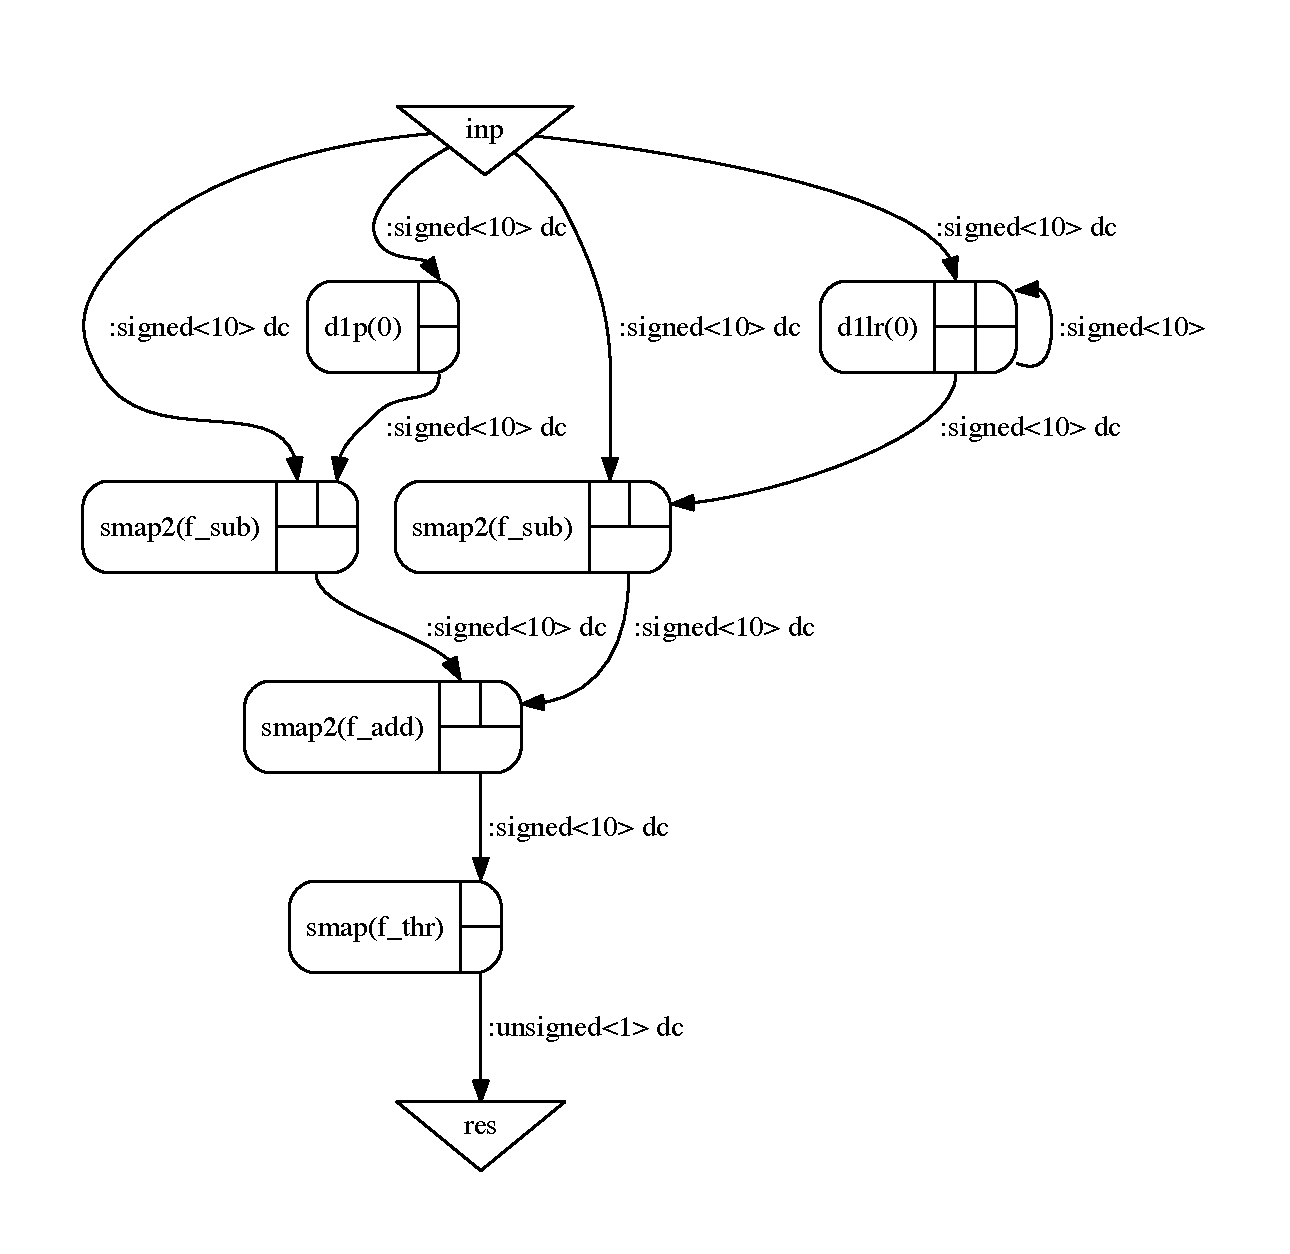
\includegraphics[width=0.75\textwidth]{figs/grad-net2}
  \caption{The data-flow graph derived from the program in listing~\ref{lst:grad-ex2} (to be
    compared with figure~\ref{fig:grad-net}}
  \label{fig:grad-net2}
\end{figure}

%%% Local Variables: 
%%% mode: latex
%%% TeX-master: "caph"
%%% End: 
